% Issues with TO derivation in paper
% 	1. Sign error for D alpha^T term in eqn S9.
% 		Li-Yan's expression differs from that in Le Kien et al by this particular factor
% 	Introduction of two TOs, then assuming they are similar...
% 		Effect of V and T offsets is to shift by XXX
% 		Still linear but not 'close'
\newcommand{\fto}{f_\mathrm{TO}}

\chapter{Precision measurement of the 413nm tune-out wavelength}
\markboth{\thechapter. MEASUREMENT OF THE 413nm TUNE-OUT}{}
\label{chap:tuneout}


	\begin{flushright}
	{\emph{``Turn on\\
			Tune in\\
			Drop out"\\} 
	Tim Leary\footnote{Leary lamented misinterpretations of this motto, coined in several of his public appearances \cite{LearyNote}}}
	\end{flushright}
	% \end{adjustwidth}

	\dropcap{Silence} has ever been a muse for the poet, but the nature of the muse is evanescent and elusive: nothing in the universe is truly motionless, as imposed by the ineradicable zero-point energy and uncertainty principle.
	But atoms in motion may undisturbed by the electric field if it oscillates at a zero crossing in the scattering cross-section.
	This chapter concerns the measurement such a \emph{tune-out} point near 413 nm \cite{Henson13,Mitroy13}.
	Here, in keeping with the tendency in metrology, I quantify this point by the tune-out \emph{frequency}, or simply use the term \emph{tune-out}. In this chapter I use the notation $L-U_1/U_2$ to specify a tune-out point by the occupied state $L$ followed by the two transitions $U_1$,$U_2$ which dominate the polarizability at the specified tune-out. In this case, the $\MetastableState \rightarrow 3^{3\!}S_1 $ transition is neglected as it is extremely weak \cite{Thomas20}. 


	
\section{Background}

	\subsection{\todo{QED and the proton radius}}
	\todo{Rewrite}
		Quantum electrodynamics (QED) describes the interaction between matter and light. It is so ubiquitous that the theory is considered a cornerstone of modern physics.
		QED has been remarkably predictive in describing fundamental processes, such as spontaneous emission rates of photons from atoms and the anomalous electron magnetic moment \cite{Aoyama15}.
		Despite QED being one of the most stringently tested theories underpinning modern physics, recent precision atomic spectroscopy measurements have uncovered several small discrepancies between experiment and theory.  
		As the precision of atomic spectroscopy approaches the part-per-trillion level, discrepancies between such predictions and experiments have come to light, such as the `proton radius puzzle'. Spectroscopic measurements (of $\mu+p$ \cite{Pohl10}, H \cite{Bezginov19,Beyer17}, and $\mu +2p$ \cite{Pohl16}) yield determinations of the proton radius which disagree by up to five standard deviations with other approaches (e+p scattering \cite{Zhan11}, and H spectroscopy\cite{Fleurbaey18}). 

		Helium is an exemplary testing ground for QED because its simple two-electron structure makes high-precision predictions tractable and testable. Notably helium also presents a nuclear `puzzle', with precision measurement of isotope shifts of the \(\MetastableState \rightarrow \LowerStates \) \cite{Zheng17} and \(\MetastableState \rightarrow \SingletState \) \cite{Rengelink18} transitions disagreeing at two standard deviations in the derived nuclear charge radius. These `puzzles' raise the possibility that the issue lies with QED itself \cite{Hill17}. Thus, we look to challenge QED directly by precision spectroscopy in helium beyond the usual energy interval measurements.

		One particularly powerful experimental observable that tests QED independently of traditional energy level measurements is the `tune-out' frequency, where the dynamic polarizability vanishes and the atom does not interact with applied laser light.  
	In this work we measure the tune-out of the metastable $\MetastableState$ state of helium (denoted He*) which lies between transitions to the $\TOLowerStateManifold$ and $\TOUpperStateManifold$ manifolds (denoted $\TO$) at approximately 726~THz (413~nm). We chose this particular tune-out frequency as the two neighbouring transitions are more than an octave apart in frequency, causing the gradient of atomic polarizability with optical frequency to be very small at the tune-out. Hence, this tune-out frequency is especially sensitive to higher order QED effects. We achieve a 20-fold improvement in the precision over the sole previous measurement \cite{Henson15}.
	For an unambiguous comparison we also present a new theoretical estimate of the \(\TO\) tune-out in helium. The experimentally determined value of 725\,736\,700\,$(40_{\mathrm{stat}},260_{\mathrm{syst}})$~MHz is within \({\sim} 2.5\sigma\) of the theory (725\,736\,053(9)~MHz), and importantly resolves both the QED contributions (\({\sim} 30 \sigma\)) and novel retardation corrections (\({\sim} 2 \sigma\)).


\subsection{Tune-out points}

	\todo{Classical oscillator intuition. Dipole force recap and extension. Why the real part? Go all the way to defining $\fto(-1,0)$ but save the ellipsometry for later. Perhaps: Materials analogy, susceptibility/polz/etc}

	An atom in an optical field experiences an energy shift in proportion to the real part of the frequency dependent polarizability, a fundamental atomic property dictated by the position of energy levels and the strengths of transitions to them (Fig. \ref{fig:schematic}). 
	A ‘tune-out’ frequency ($f_\mathrm{TO}$) occurs between transition frequencies at the point where the contributions to the dynamic polarizability [$\alpha(f)$] by all transitions below that frequency are balanced by all those above it ($\alpha(f)=0$) \cite{LeBlanc07}. 
	This balance point is hence fixed by the strength and frequency of every transition in the atomic spectrum and thus provides a precise constraint on the ratio of transition dipole matrix elements. 

	\begin{figure} 
		\centering
		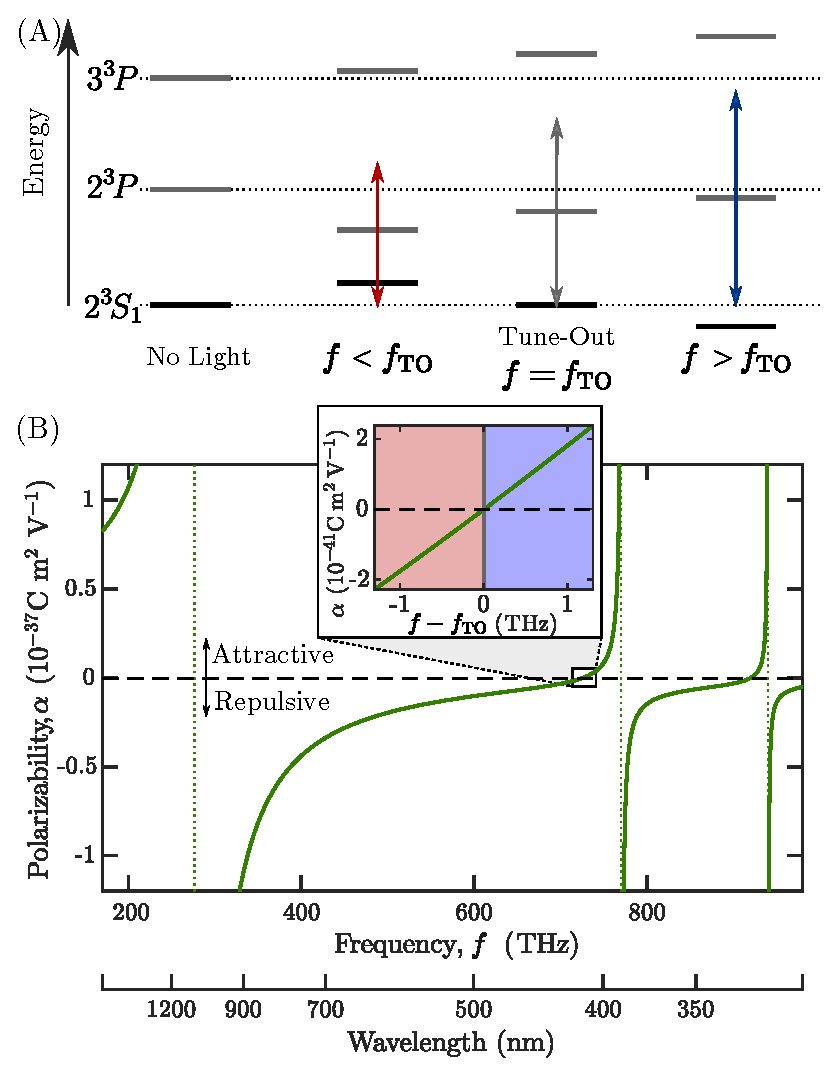
\includegraphics[width=\textwidth]{fig/tuneout/composite_polz_fig}
		\caption{\textbf{Tune-out in atomic helium:}
		(A) Atomic energy level shift of the dominant state (manifolds) about the tune-out.  When an optical field of frequency $f$ (arrows) is applied to the atom the individual
		levels shift dependent on the difference between $f$ and the transition frequency. At the tune-out frequency $f_{\mathrm{TO}}$ (middle right), the shifts to the $\MetastableState$ state energy cancel.
		Energy spacing and shifts not to scale.
		(B) Theoretical frequency dependent polarizability of $\MetastableState$ helium, for a constant light polarisation, indicating that the polarizability vanishes near 726~THz, - the tune-out frequency measured in this paper. 
		Vertical dotted lines show, from left to right, the transitions to the  $\TOLowerStateManifold$, $\TOUpperStateManifold$,$4^{3\!}P$ manifolds. Inset shows the approximately linear polarizability with frequency about the tune-out.
		}
		\label{fig:schematic} 
	\end{figure}


\subsubsection{Magic wavelengths}
	It bears noting that tune-out points are associated with \emph{states} of the atom, where the stark shift $\Delta E_\mathrm{Stark} =0$.
	A distinct but related concept is `magic wavelengths' which are associated with \emph{transitions} between states and defined by the point where the differential dynamic polarizability (or differential stark shift) vanishes $\Delta E_\mathrm{Stark,Upper}-\Delta E_\mathrm{Stark,Lower}$. 
	Magic wavelengths have attracted a great deal of interest for their utility in constructing optical lattice clocks \cite{Takamoto05,Derevianko11} by decoupling the Stark shift of the clock transition from the intensity of the trapping beams.
	A major technical issue in atom- and ion-based frequency references is the calculation of the Stark shift due to black-body radiation from the vacuum chamber containing the test system \cite{Fasano21}.
	Precision measurements of magic wavelengths constrain models of the polarizability over large spectral ranges and thus serve to characterize and help suppress black-body shifts in these systems \cite{Chanu20,Fasano21}.			
	While magic wavelengths are presented by Nature to the scientist, it is also possible to emulate the effect of a magic wavelength by using an additional laser to counteract the Stark shift from a trapping or probe beam \cite{Hilton19}.
	Recent progress has also overcome the higher-order effects beyond the electric dipole (namely the magnetic dipole, electric quadrupole, and hyperpolarizability effects) by precisely tuning the magic-wavelength trap to a `magic intensity' and achieving a Stark-shift cancellation to the $10^{-19}$  level in a Strontium latttice clock \cite{Ushijima18}.
	Precision frequency measurements using neutral atoms (and ions \cite{Chanu20}) in optical lattices continue to provide constraints on possible variations in fundamental constants across space and time \cite{Uzan03,Blatt08,Huntemann14} and have been identified as compact detectors for gravitational waves \cite{Kolkowitz16} and dark matter candidates \cite{Derevianko14}.
	Further, matter-wave guides built using magic wavelengths provide advantages for atom-interferometric gradiometry of gravitational and electromagnetic fields \cite{Akatsuka17}
	Finally, magic (and indeed tune-out) wavelengths have recently been reported for ultracold diatomic molecules, thus extending the suite of control options available at the frontier of ultracold matter sciences \cite{Bause20}.
	\todo{Comment on difference between magic and tune-out lattices for qsim/control}
		strontium state-dependen lattice
		looks like a good read
		https://pure.mpg.de/rest/items/item_3322534/component/file_3322535/content 

	Magic wavelengths are, of course, also of interest for their potential use in tests of basic atomic structure theory.
	Highly precise measurements of magic wavelengths have been used to determine transition matrix elements in Rubidium to better than 0.1\% \cite{Herold12}.
	For comparison, tune-out measurements in rubidium have yielded the ratio of oscillator strengths (rather than their absolute values) with accuracy at the $10^{-4}$ level \cite{Leonard15}.
	However, most magic wavelength measuremente are made using heavy elements like Strontium , Barium \cite{Chanu20}, Mercury \cite{Yi11}, Rubidium \cite{Herold12}, and Cesium \cite{Yoon19}, whose complex internal structure restricts the accuracy with which these wavelengths can be predicted.
	For instance, while current predictions of magic wavelengths in heavy elements are yet to reach the parts-per-million level, calculations for Helium are already at this level\cite{Wu18,Zhang21_magic}.
	While the contribution of QED effects are included for these helium magic wavelengths, their contribution is generally smaller than the theoretical uncertainty associated with the individual energy levels and thus are not yet ready for comparison with experiments.
	However, a very recent work identified the 1335 nm magic wavelength as a candidate for tests of atomic structure theory due to its sensitivity to the finite nuclear mass, and relativistic and QED effects \cite{Zhang21_magic} (contributing to the wavelength at the level of 232, 247, and 21 ppm respectively).
	A measurement of this wavelength to 0.01 nm precision (fractional error $\sim10^{-5}$) would suffice to check the predicted QED contributions.
	Indeed, magic wavelengths have already found use in tests of QED with helium, albeit through their role as dipole traps for precision measurements of forbidden transition energies \cite{Regnelink18}.
	A further application to helium was recently proposed wherein one uses a 1265 nm magic wavelength optical trap while another 934 nm magic wavelength beam provides the first of two photons for dicrhoic excitation of the  forbidden $2\triplet S_1\rightarrow 3\triplet S_1$ transition near 427.7 nm \cite{Thomas20, Zhang21_forbidden}.
	This would reduce the effect of the main systematic uncertainty (the AC Stark shift) from 5 MHz to below 100 kHz.

% From Li-Yan's document (helium.pdf); the dynamic polarizability is $\alpha_1(\omega) = \sum_n \frac{f_{0n}}{\Delta E_{0n}^2 - \omega^2}$ in terms of all those oscillator strengths

\subsection{Other TO measurements}
	\begin{itemize}
	\item \todo{Read these past measurements}
	\item \todo{Make first paras a summary of method, incl. identifying f(-1,0), and then outline the rest of the section as detailed discussions of the key points}
	\item\todo{Relationship to magic wavelengths, etc etc}
	\end{itemize}
	2015 safranova theoretical identification of TO wavelengths in Strontium, check their accuracy
		Ref for extracting transition rates
		https://journals.aps.org/pra/abstract/10.1103/PhysRevA.92.040501

	2011 TOs for alkali metals, v early theory work
		https://journals.aps.org/pra/abstract/10.1103/PhysRevA.84.043401
	2013 Cheng calculations of TOs for alkali-earth metals
		https://journals.aps.org/pra/abstract/10.1103/PhysRevA.88.022511
	2013 Jiang prediction of TO wavelengths for potassium
		https://journals.aps.org/pra/abstract/10.1103/PhysRevA.87.032518
	2016 Wang tune-outs in R, high precision measurements to 790.018187(193) and 790.032602(193) nm
		Agree with theory (Leonard 15)
		https://journals.aps.org/pra/abstract/10.1103/PhysRevA.94.052510
	2016 Schmidt 790nm tuneout in Rb by KD scattering of a BEC
		790.01858(23) nm with sub-pm accuracy
		https://journals.aps.org/pra/abstract/10.1103/PhysRevA.93.022507
	2016 Dammalapati calcs of magic and TOs for francium
		https://journals.aps.org/pra/abstract/10.1103/PhysRevA.93.043407
	2017 Trubko Potassium TO 768.9701(4) nm using atom interferometry
		 Ratio of oscillator strenghts inferred 2.066(11), ratio of line strenghts 1.9977(11)
		https://journals.aps.org/pra/abstract/10.1103/PhysRevA.95.052507
	2017 Kao Dysprosium TO measurement, reported to the percent level, using kapitza-dirac diffraction
		https://www.osapublishing.org/oe/fulltext.cfm?uri=oe-25-4-3411&id=359890 
	2017 Leonard high precision Rb tune-out measurement
		erratum: Actual value = 790.032 326(32) nm, matrix element ratio 1.992 17(3)
		theoretical value 790.0315(7) (after correction)

	2018 Tang predictions of Thallium TO and magics
		https://journals.aps.org/pra/abstract/10.1103/PhysRevA.98.062511
	2019 Copenhaver 7Li tune-out measurement with atom interferometry
		 3329.5(1.4) MHz for the tensor-shifted tune out  with σ± light polarization and 3310.6(4.9) MHz with scalar polz
		 good ref for distinction between terms
		https://journals.aps.org/pra/abstract/10.1103/PhysRevA.100.063603
	2020 Decamps 671nm TO for 7Li by atom interferometry
		Can be corrected (via tensor terms) to agree with Copenhaver et al
		https://journals.aps.org/pra/abstract/10.1103/PhysRevA.101.033614
	2020 Jian tune-out wavelength for 133Cs
		Calculation - check precision, and note that tensor part is very very small in this case
		https://journals.aps.org/pra/abstract/10.1103/PhysRevA.102.042823
	2021 Jiang tuneouts for Ba+ ions
		Precision looks quite good
		Sensitive to QED?
		https://journals.aps.org/pra/abstract/10.1103/PhysRevA.103.032803


	
	
	As a test of QED, a tune-out frequency is advantageous because it is a null measurement, which does not require calibration of the light intensity or a measurement of excitation probability. These factors have previously limited the precision of direct transition strength measurements \cite{Boloufa09,Vogt07,Thomas20}. In comparison, previous tune-out measurements have been successful in measuring QED effects \cite{Leonard15,Holmgren12,Schmidt16,Herold12,Henson15}.



\subsection{QED prediction of the tune-out point}
	% theory work
	\todo{Compress, be clearer it's a summary, acknowledge theorists. Prioritize reformulation as zero in rayleigh scattering cross section.}
	Following the first prediction \cite{Mitroy13} and measurement \cite{Henson15} of the tune-out, a vigorous campaign of theoretical studies \cite{Zhang16,ManaloThesis,Drake19,Zhang19, Pachucki19} has reduced the uncertainty in the predicted frequency, which limited comparison with experiment. In parallel with work at ANU, our collaborators improved on the state-of-the-art calculation \cite{Zhang19} of the tune-out frequency by accounting for finite nuclear mass, relativistic, QED, finite nuclear size, negative energy states, and finite wavelength retardation effects \cite{Drake19, Pachucki19,ArxivTO}. These calculations were done using the non-relativistic QED method and improve the precision of the state of the art by an order of magnitude with an uncertainty smaller than that obtained in the measurement in this chapter. The work is briefly described in this section, and presented in more detail in \cite{ArxivTO}.


	The nr-QED method consideres the nonrelativistic Schr\"odinger equation and includes terms for the Breit interaction by perturbation theory \cite{BetheSalpeter,Piszczatowski15,Puchalski16,Puchalski20}.  The dynamic polarizability is expressed to second order in the interaction with an electromagnetic field of frequency $\omega$, and contributions from relativistic and QED effects enter through an additional perturbation.  
	
	 In the electric dipole approximation, the frequency-dependent dipole polarizability is given by 
	  \begin{equation}
	  \bar{\alpha}_{\rm d}(\omega) = \frac12[\alpha_{\rm d}(\omega) + \alpha_{\rm d}(-\omega)],
	  \end{equation}
	  where
	\begin{equation}
	\alpha_{\rm d}(\omega) = 2\langle\psi_0|\edotr{\cal R}(\omega)\edotr|\psi_0\rangle,
	\end{equation}
	which is in turn defined in terms of the resolvent operator
	\begin{equation}
	{\cal R}(\omega) = Q(H_0 - E_0 + \hbar\omega)^{-1}Q,
	\end{equation}
	where $H_0$ is the field-free Hamiltonian, $E_0$ is the unperturbed energy of the $2^3S_1$ state, and $Q = 1 - |\psi_0\rangle\langle \psi_0|$ is a projection operator.  

	$\mbox{\boldmath{$\hat{\rm e}$}}$ is a polarization vector pointing in the direction of the electric field, and ${\bf r} = {\bf r}_1 + {\bf r}_2$.  
	Additional time-independent perturbations $\hat{X}$ are packaged into a term labeled $\delta\alpha_{\rm d}^{\hat{X}}(\omega)$
	The tune-out frequency $\omega_{\rm TO}$ is defined by the condition
	\begin{equation}
	\label{eq:baralpha}
	\bar{\alpha}_{\rm d}(\omega) + \sum_{\hat{X}} \delta\bar{\alpha}_{\rm d}^{\hat{X}}(\omega) +
	\delta\bar{\alpha}_{\rm d}^{\partial_{\cal E}^2\ln k_0}(\omega) = 0
	\end{equation}
	where the sum runs over all the perturbations ($\hat{X}$) in the calculation, and $\delta\bar{\alpha}_{\rm d}^{\partial_{\cal E}^2\ln k_0}(\omega)$ is an additional QED correction due to the field dependence of the Bethe logarithm. The included relativistic corrections are the spin-independent terms, the orbit-orbit interaction, and the  spin-dependent spin-spin interaction, and the Darwin term (see \cite{ArxivTO} for definitions and calculation of the aforementioned terms).

	\begin{table}[t]
	\centering
	%\vbox{\hsize 5.2in \noindent
	% \begin{ruledtabular}
	\begin{tabular}{l r r}
	Quantity    &Value (MHz) & Uncertainty (MHz) \\
	\hline
	\multicolumn{3}{c}{\textbf{Nonrelativistic and Relativistic terms}} \\
	Nonrelativistic (NR) & 725\,645\,115& 2       \\
	NR + relativistic scalar $(\alpha^{\rm S})$    & 725\,742\,216&6   \\
	Relativistic tensor $(-\frac12\alpha^{\rm T})$ &   1\,755& \\
	\hline
	Total non-QED        & 725\,743\,950&6     \\
	\hline
	\multicolumn{3}{c}{\textbf{QED terms}} \\
	QED $\alpha^3$       &       -7\,298& 1       \\
	QED $\alpha^4$       &          -127& 6       \\
	\hline
	Total QED            &         -7\,425& 8     \\
	\hline
	Retardation          &          -477 &        \\
	Nuclear size         &             5&          \\
	\hline
	Grand total          & 725\,736\,053& 9       \\
	Experiment           & 725\,736\,700& 260 \\
	\hline
	Difference           &          -647& 260\\
	\end{tabular}\\
	\caption{\label{tab:theory}Summary of theoretical contributions to the helium $\TO$ manifold tune-out frequency near 725.7 THz.}
	% \end{ruledtabular}
	\end{table}
	QED corrections are included in the form of effective operators up to fourth order in $\alpha$ \cite{Yerokhin10}, including the Araki-Sucher terms \cite{Araki57,Sucher58} ($\alpha^3$) and radiative QED terms ($\alpha^4$). The remaining nonradiative terms, amounting to about 5\% of the contributions from the radiative terms for the $2^3S_1$ state \cite{Piszczatowski2015,Pachucki2006}, result in an uncertainty of about 6MHz and are considered the dominant uncertainty.	A significant contribution of the theoretical work is the inclusion of retardation corrections recently derived by Pachucki and Puchalski \cite{Pachucki19,Drake19}.  These additions represent a reformulation of the problem as a zero in the coherent Rayleigh scattering amplitude for an atom in free space, instead of a zero in the frequency-dependent polarizability for an atom in an optical lattice \cite{Pachucki19,Drake19}. 


	The results are presented in Table~\ref{tab:theory}. The entries from nonrelativistic, relativistic, and QED contributions are not strictly additive because changing one effect, such as the relativistic correction, changes the tune-out frequency at which the other effects are evaluated.  Thus the first entry is the nonrelativistic tune-out frequency with finite nuclear mass effects included.  The next entry is the scalar part of the relativistic correction arising from the higher terms in the Breit interaction.  The entry from the spin-spin interaction (1755~MHz) is entirely responsible for the tensor part of the tune-out frequency (excluding the Schwinger radiative correction term $\alpha/\pi$).  These terms determine the nonrelativistic and relativistic part of the tune-out frequency.  The remaining terms are small enough that they can be added linearly.  The leading QED correction of order $\alpha^3$ ($-7298(6)$ MHz) includes the anomalous magnetic moment correction (8 MHz) and the very small estimate of $-0.124(3)$ MHz for the $\delta\bar{\alpha}_{\rm d}^{\partial_{\cal E}^2\ln k_0}$ term.  The terms of order $\alpha^4$ include only the radiative corrections.  The dominant source of uncertainty is thus the remaining nonradiative terms not included in the calculation, but which were previously computed for the $2^3S_1$ state energy \cite{Pachucki06}.  The remaining terms are the retardation correction of $-477$ MHz and a finite nuclear size correction.



\section{Measurement technique}
	\label{sec:trap_freq_measure}
	\todo{Ensure one has the $2\pi$s in the right places; I think I use rad hz here}


	\begin{figure}
	\begin{minipage}{0.5\textwidth}
	\vspace{0pt}
	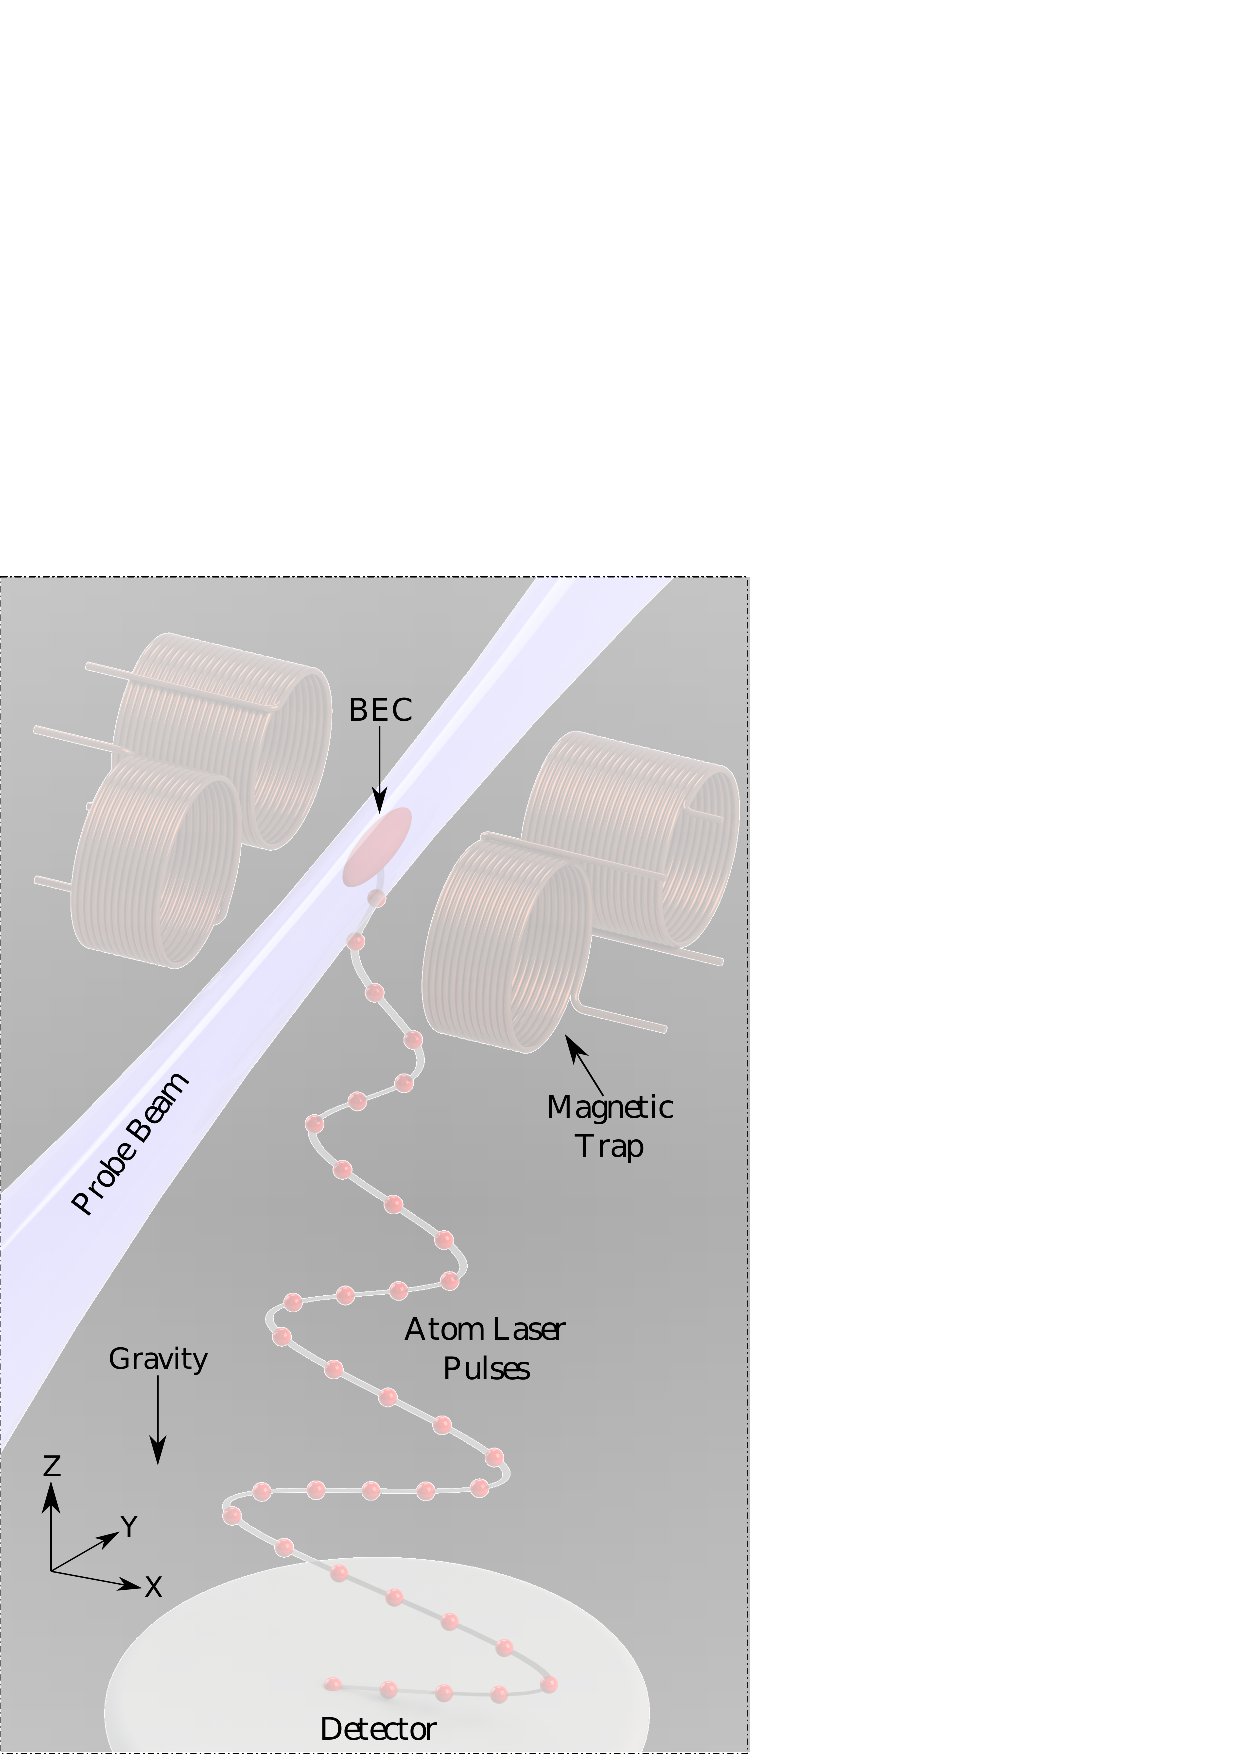
\includegraphics[width=\textwidth]{fig/tuneout/exp_schematic.png}
	\end{minipage}
	\hfill
	\begin{minipage}{0.5\textwidth}
	\vspace{0pt}
	\caption{
	Method to determine the tune-out for a fixed probe beam polarization. a magnetically trapped BEC of metastable helium atoms is illuminated with a probe laser beam with an adjustable (optical) frequency. A sequence of atom laser pulses is outcoupled from the BEC to sample the oscillation. \todo{Longer caption text. Integrate with this section.}
	}
	\label{fig:exp_schematic} 
	\end{minipage}
	\end{figure}


	To determine a tune-out point is essentially to measure the frequency where the optical dipole potential  vanishes.
	In our measurement, we quantified the shift in the transverse trapping frequency $\omega_x$ when the magnetic trap was overlapped with a probe laser beam (see Fig. \ref{}). 
	The potential energy is then given by the sum of both a harmonic magnetic potential and a Gaussian optical potential,
	\begin{equation}
		U_\mathrm{net} = U_{\mathrm{trap}} + U_\mathrm{dip},
	\end{equation}
	where the magnetic trapping potential takes the form
	\begin{equation}
		U_\mathrm{trap} = \frac{m}{2}\left(\omega_{x}^{2}x^2+\omega_{y}^{2}y^2+\omega_{z}^{2}z^2 \right)
	\end{equation}
	and the dipole potential is given in general by (see section \ref{sec:dipole} and \cite{Grimm00})
	\begin{align}
	    U_{\mathrm{dip}}=-\frac{1}{2 \epsilon_{0} c} \operatorname{Re}(\alpha) I.
	\end{align}
	For a Gaussian beam which is aligned with the weak ($x$) axis of the trap and focuses $P$ watts of power to a spot size $w_0$, the intensity profile is 
	\begin{equation}
	    I_{\mathrm{dip}} =
	        \frac{2 P}{\pi w_0^2} \left(\frac{w_0}{w(x)}\right)^2 \exp\left( -\frac{1}{2} \frac{(y^2+z^2)}{w(x)^2} \right)
	 \end{equation}
	 where $w(x) = w_0\sqrt{1+(x/x_R)}$ is the waist size at a position $x$ along the beam axis and $x_R$ is the Rayleigh length. 
	 In the small-amplitude oscillation limit we can consider the total potential to be harmonic and retain only the terms up to second order in a Taylor expansion. If we further assume that the trapped BEC oscillates in the $y$ direction only then we can write the potential along the direction of motion as
	 \begin{equation}
	 U_\mathrm{net} \approx -\frac{\mathrm{Re}(\alpha)  P}{\pi 
   c {w_0}^2 \epsilon} + \left(\frac{2 \mathrm{Re}(\alpha)  P}{\pi  c {w_0}^4 \epsilon }+\frac{m {\omega_y}^2}{2}\right) y^2
	 \end{equation}
	 when evaluated about $x=z=0$.
	 Noting that the restoring force for a harmonic oscillator is given by $F_y = -\partial_y U_\mathrm{net} = -k_\mathrm{net} y$, we can identify the perturbed trapping frequency via the spring constant $k_y$:
	 \begin{align}
	 	\omega_\mathrm{net} &= \sqrt{\frac{k_\mathrm{net}}{m}}\\
	 	&= \sqrt{{\omega_y}^2+\frac{4 P \mathrm{Re}(\alpha)}{m c \epsilon w_{0}^4}}
	 \end{align}
	wherein we can identify the trap and probe frequency contributions by setting $P=0$ and $\omega_y=0$, respectively. 
	We thus obtain 
	\begin{equation}
		\omega_\mathrm{probe} = \sqrt{\frac{4 \mathrm{Re}(\alpha)  P}{m c \epsilon w_{0}^4}}
	\end{equation}
	and have the relation
	\begin{align}
		\omega_\mathrm{net}^2 &= \omega_\mathrm{trap}^2 + \omega_\mathrm{probe}^2\\
		&= \omega_\mathrm{trap}^2 + \frac{4   P}{m c \epsilon w_{0}^4}\mathrm{Re}(\alpha)
	\end{align}
	which shows that the squared shift in trapping frequency $\omega_\mathrm{probe}^2 = \omega_\mathrm{net}^2 - \omega_\mathrm{trap}^2$ is linear in the probe power and the polarizability. 
	An immediate corollary is that if the probe beam power is stabilized then $\omega_\mathrm{probe}^2$	is linear solely in $\mathrm{Re}(\alpha)$. Recalling that the dynamic polarizability $\alpha(f)$ depends on the light frequency $f$, is follows that ascertaining the frequency at which $\omega_\mathrm{probe}=0$ constitutes a determination of the tune-out point.
	This result is the basis of the measurement method, along with one further assumption: that the polarizability is linear with detuning from the tune-out.

\subsection{Polarizability near $\fto$}

	% in \cite{LeKien13}
	% [17,18,20] scalar and tensor polz calculated for Sr and [21,22] For Cs motivated by calculation of magic wavelengths
	% [16] variety of ways to calculate polarizabilities
	% [17-19] magic wavelengths are those for which both upper and lower states of a transition are shifted by equal amounts 
	% [23,24] tune-out wavelength searches for alkali-metal atoms
	% [25] there are three components, scalar tensor and vector
	% [33] calc sof SVT polz for Rb
	% [37] imaginary part of polz is related to the scattering rate

	The time-dependent polarization of an atom in response to a time-varying electric field is governed by the dynamical polarizability \cite{LeKien13,etc}.
	The dynamical polarizability determines the size of the Stark shift of all the states in an atom and thus is of quite general interest in the context of cold-atom sciences.
	The dynamical polarizabilities for alkali-metal atoms and other species (?) have been calculated, usually motivated by the search for magic wavelengths.
	Magic wavelengths are those where the upper and lower states of a transition are Stark-shifted by identical amounts and thus the transition energy in the presence of light is identical to that where there is no background light.
	Such wavelengths are of interest for clocks and lattices \cite{somepapers}.
	By comparison, the tune-out is a point where the Stark shift of a \emph{level}, rather than a \emph{transition}, vanishes. 
	Both features of the atomic response can be captured in the same framework for describing the interaction of an atom with an electric field
	\begin{equation}
		\mathbf{E} = \frac{1}{2}\mathbf{\mathcal{E}}e^{-2\pi i f t}+\mathrm{c.c.}
	\end{equation}
	where $\mathbf{\mathcal{E}}=\mathcal{E}\mathbf{u}$ is the electric field envelope with magnitude $\mathcal{E}$ and polarization vector $\mathbf{u}$ (both of these terms may be complex).
	For a far-off-resonant light field, the Stark shift will be small compared with the fine-structure level splitting. 
	In this case, and working in the dipole appoximation, the interaction between the atom and the light field is captured by the operator
	\begin{equation}
		\Delta E_\mathrm{Stark} = -\frac{1}{2}\left(\mathcal{E}\mathbf{u}\cdot\mathbf{d}e^{-2\pi i f t} - \mathcal{E}^*\mathbf{u}^*\cdot\mathbf{d}e^{2\pi i f t}\right),
	\end{equation}
	which, after a lengthy derivation (see \cite{LeKien13}) can be written as
	\begin{align}
		\Delta E_\mathrm{Stark} &= -\frac{1}{2\epsilon_0 c} \mathrm{Re}(\alpha(f)) I\\
		&=-\frac{1}{4}|\mathbf{\mathcal{E}}|^2\left(\alpha^S + C\alpha^V \frac{m_J}{2J} - D\alpha^T\frac{3m_{J}^{2}-J(J+1)}{2J(2J-1)}\right)
	\end{align}
	% note I = c \epsilon_0 |E|^2/2 so the first line is just Re(a)E^2/4
	\todo{is there a factor of 2 missing here?} for a state with total angular momentum $J$ with a $z$-projection of $m_J$. The step between the two lines uses the definition of electric field intensity $I = 2\epsilon_0 c|\mathcal{E}|^2$. For brevity, and as we are concerned solely with the real part of the polarizability\footnote{The imaginary part of $\alpha$ pertains to the photon scattering rate through $\Gamma_\mathrm{sc} = \mathrm{Im}(\alpha)I/\hbar\epsilon_0 c$ \cite{LeKien13,Grimm00}.}, we will simply use the notation $\alpha(f)$ to refer to the \emph{real} part of the polarizability. From the preceding equation one then obtains the polarizability for the $2\triplet S_1(m_J=1)$ state:
	\begin{equation}
		 \alpha(f) = \alpha^S(f) + \frac{1}{2}\left(C\alpha^V(f)  - D\alpha^T(f)\right)
		 \label{eqn:master_polz}
	\end{equation}
	Where frequency-dependent scalar, vector, and tensor polarizabilities are $\alpha^S$, $\alpha^V$, and $\alpha^T$, respectively, and the coefficients $C = 2\mathrm{Im}(u_{x}^*u_y)$ and $D = 1 - 3|u_z|^2$ depend on the polarization vector $\mathbf{u}$ relative to the quantization axis of the atom, denoted $z$. 
	We will deal with the polarization effects shortly, but note for now that they are bounded by $C\in[0,2]$ and $D\in[-2,1]$, and return to the frequency-dependent effects.
	Expanding the preceding equation about some frequency $f_0$ near $\fto$ we have
	\begin{align}
		 \alpha(f)  \approx & \alpha^S(f_0) + (f-f_0)\frac{d\alpha^S}{df}\Bigr|_{f=f_0} \\
		 &+ \frac{C}{2}\left(\alpha^V(f_0) + (f-f_0)\frac{d\alpha^V}{df}\Bigr|_{f=f_0} \right)\\
		 &-\frac{D}{2}\left(\alpha^T(f_0) + (f-f_0)\frac{d\alpha^T}{df}\Bigr|_{f=f_0} \right)
	\end{align}
	It is expected on theoretical grounds that the vector and tensor polarizabilities are nearly constant over the scan ranges we use in this experiment \cite{ArxivTO}.
	Hence, we can drop the respective derivative terms and arrive at

	\begin{align}
		 \alpha(f)  \approx & \alpha^S(f_0) + \frac{C}{2}\alpha^V(f_0) -\frac{D}{2}\alpha^T(f_0) +  \frac{d\alpha^S}{df}\Bigr|_{f=f_0} (f-f_0).
	\end{align}
	The condition that $\alpha(\fto)=0$ implies
	\begin{align}
		 \frac{d\alpha^S}{df}\Bigr|_{f=f_0} (\fto-f_0) \approx & -\alpha^S(f_0) - \frac{C}{2}\alpha^V(f_0) +\frac{D}{2}\alpha^T(f_0)
	\end{align}
	and hence
	\begin{align}
		 \fto \approx & f_0 + \alpha^S(f_0) - \frac{C}{2}\beta^V(f_0) +\frac{D}{2}\beta^T(f_0)
	\end{align}
	where 
	\begin{equation}
		\beta^V(f) = \alpha^V(f)\left(\frac{d\alpha^S}{df}\Bigr|_{f=f_0}\right)^{-1}
	\end{equation}
	and similarly for $\beta^T$.
	It can be seen that the tune-out frequency thus depends on the polarization of the light through $C$ and $D$ while the gradient of the polarizability at this point is dominated by the scalar polarizability. 
	As these coefficients themselves are bounded, the size of the effect is determined by the values of $\alpha^V(\fto)$ and $\alpha^T(\fto)$, which lead to a shift in the tune-out frequency of  \todo{VALUE} and 3.51 GHz, respectively\footnote{Conveyed by L. Y. Tang and G. W. F. Drake in personal communication during the course of research}.
	% Tang: When A cos \theta_k is adjusted from -1 to 1 the TO shifts by 0.4-6 pm 
	We must specify a quantity in order to make an unambiguous comparison with theoretical calculations, and thus far we have only manifold of possible values subject to the constraint that $\mathbf{u}^*\cdot\mathbf{u}=1$.
	We can do this in such a way that eliminates the large effect of $\alpha^V$ by exploiting the interrelationship between the components of $\mathbf{u}$.

	% could continue by expanding about \fto^S and then finding a more general condition for \fto in terms of \fto^S and the other alphas, more like in paper. But what is the point here, really? Time to work thorugh the polz at last...

\subsubsection{Polarization-dependent tune-out points}


	We take a short detour here to build up the language necessary to discuss the role of polarization in determining the tune-out frequency.
	The following works in a semiclassical framework, wherein the atom is described in a quantum-mechanical way and a monochromatic electric field takes on a classical state as
	\begin{equation}
		\vec{E}(\mathbf{r},t) = \mathcal{E}(\mathbf{r},t)\hat{\mathbf{u}}(\mathbf{r}),
	\end{equation}
	where $\hat{\mathbf{u}}$ is the unit polarization vector. The electric field propagates in the direction of the Poynting vector $\mathbf{S} = \mathbf{E}\times\mathbf{B}$, and hence we have $\hat{\mathbf{u}}\perp\mathbf{S}$. Therefore, if we fix $z'$ as the propagation direction (i.e. along the beam axis, we will relate the dashed coordinates to the lab frame shortly) then we can write the electric field in the coordinates $(x',y',z')$ as 
	\begin{equation}
		\vec{E}(\mathbf{r},t) = \begin{bmatrix}E_{x'}e^{i\phi_{x'}}\\
												E_{y'}e^{i\phi_{y'}}\\
												0)
												\end{bmatrix}e^{i(kz'-2\pi f t)}
	\end{equation}
	One can then consider first two components, also known as the \emph{Jones vector} which captures the amplitude and relative phases in the $x'$ and $y'$ direction.
	Rather, we will work with the \emph{normalized} Jones vector 
	\begin{equation}
	\mathbf{j} = \begin{bmatrix}\mathbf{u}_{x'}e^{i\phi_{x'}}\\
								\mathbf{u}_{y'}e^{i\phi_{y'}})\end{bmatrix}
	\end{equation}
	which captures the 


	  - a decision which clarifies much of the working below.
	First, notice that in this two-dimensional notation, we can write the horizontal/vertical, diagonal/antidiagonal, and right-circular/left-circular polarization states as follows:
	
	\todo{Fix table}

	% \begin{tabular}{l l}
	% 	% $\mathbf{h} = \begin{bmatrix}1\\0\end{bmatrix}$ & $\mathbf{v} = \begin{bmatrix}0\\1\end{bmatrix}$\\
	% 	$\mathbf{d} = \frac{1}{\sqrt{2}}\begin{bmatrix}1\\1\end{bmatrix}$ & $\mathbf{a} = \frac{1}{\sqrt{2}}\begin{bmatrix}1\\-1\end{bmatrix}$\\
	% 	$\mathbf{r} = \frac{1}{\sqrt{2}}\begin{bmatrix}1\\-i\end{bmatrix}$ & $\mathbf{l} = \frac{1}{\sqrt{2}}\begin{bmatrix}1\\i\end{bmatrix}$
	% \end{tabular}
	and thus the degree of some polarization $p$ can be calculated by the overlap vector $\mathbf{u}\cdot\mathbf{p}$. 
	Second, notice that the normalized two-dimensional complex polarization vector lives in the same Hilbert space as a two-level quantum system - it is a two-dimensional Hermitian matrix with unit trace.
	Motivated by this we can construct the \emph{coherence matrix} from the Jones vector via 
	\begin{equation}
		\mathbf{\chi} = \mathbf{j}^\dagger\otimes\mathbf{j} = \begin{bmatrix} u_{x'}^2 & u_{x'} u_{y'} e^{-i(\phi_{x'}-\phi_{y'})} \\ u_{x'} u_{y'} e^{i(\phi_{x'}-\phi_{y'})} & u_{y'}^2\end{bmatrix},
	\end{equation}
	which can be written as $\mathbf{\chi} = \sum_{i=0}^3 a_i\sigma^{i}$ in terms of the Pauli basis.
	The outer product also maps the aforementioned polarization states to 

	\begin{tabular}{c c}
		${H} = \begin{bmatrix}1&0\\0&0\end{bmatrix}$ 					& ${V} = \begin{bmatrix}0&0\\0&1\end{bmatrix}$\\
		${D} = \frac{1}{{2}}\begin{bmatrix}1&1\\1&1\end{bmatrix}$ &$ {A} = \frac{1}{{2}}\begin{bmatrix}1&-1\\-1&1\end{bmatrix}$\\
		${R} = \frac{1}{{2}}\begin{bmatrix}1&i\\-i&1\end{bmatrix}$ & ${L} = \frac{1}{{2}}\begin{bmatrix}1&-i\\i&1\end{bmatrix}$,
	\end{tabular}

	thus the coherence matrix can generally be written in the form $\chi = I + \mathbf{S}\cdot\mathbf{\sigma}$ where $\mathbf{S}\in\mathbb{R}^3$ and $|\mathbf{S}|\leq1$, analogous to the expression of a qubit state as a Bloch vector.
	Completing the analogy, we note that the pairs of orthogonal polarization are related by the transformation $\mathbf{S}\rightarrow-\mathbf{S}$, that purely-polarized and unpolarized light correspond to the case $|\mathbf{S}|=1$ and $|\mathbf{S}|=0$, respectively, and that we can depict the polarization state in three real dimensions using the Poincar\'{e} sphere construction, as shown in Fig. \ref{polz_diag}.
	By convention, denote the full form of the Stokes vector $\mathbf{S} = (I,Q,U,V)$ where $I$ is the beam intensity and the latter three components are the  the degrees of linear (along $x'$ or $y'$) polarization, (anti-)diagonal polarization, and circular polarization in the frame defined by the beam axis\footnote{The construction of the Stokes vector on differs from the Bloch vector in that the former also includes the intensity of the light, which we have omitted here by working with the unit polarization vector. Including the intensity only introduces a multiplicative factor to all other coefficents and permits the trace norm to take any value. For convenience, we will persist with this abuse of notation.}.
	We can now turn attention back to the $C$ and $D$ coefficients, interpret them in terms of the polarization in the atomic reference frame, and relate the polarization state of the beam to the tune-out behaviour.

\subsubsection{Polarization in the atomic frame}
%  make diagrams like https://en.wikipedia.org/wiki/File:Polarisation_ellipse2.svg 
% https://en.wikipedia.org/wiki/File:Poincar%C3%A9_sphere.svg

	To translate between the Stokes vector selected by the experimentalist (using the pre-vaccum optics) and the Stokes vector relative to the axis of quantized angular momentum, we need the linear tranformation between their respective coordinate systems $\vec{x}'$ and $\vec{x}$. 
	We can use the simple relation
	\begin{equation}
		\mathbf{u}'_{i}=\vec{x'}_i\cdot\mathbf{u}_j
	\end{equation}
	wherein we determine the $\vec{x}'$ and $\mathbf{u}_j$ in a common $x$ basis we can use the general rotation matrix
	\begin{align}
	x =& r \sin(\phi)\cos(\theta)\\
	y =& r \sin(\phi)\sin(\theta)\\
	z =& r \cos(\phi)\\
	x' &= r' \sin(\phi')\cos(\theta')\\
	y' &= r' \sin(\phi')\sin(\theta')\\
	z' &= r' \cos(\phi')
	\end{align}
	
	\begin{align}
	R_{i,j}  &= \ket{x_i}\bra{{x_j}'}	\\
	&= \exp(J \Theta t)~\mathrm{where}\\
	\Theta&= \begin{bmatrix}
		 0 & \theta_3 & -\theta_2\\
		 -\theta_3 & 0 &\theta_1 \\
		 \theta_2 & -\theta_1 & 0
		\end{bmatrix}
	\end{align}

	where $\Theta$ is the generator of the supgroup of rotations within the Poincar\'{e} group.

	The clearest element to interpret is the value $D = 1-3|u_z|^2$, wherein the component $u_z$ is the degree of polarization along the $z$ axis. 
	The projection of the polarization vector along this axis is $\mathbf{u}\cdot\hat{z} = \cos{\theta_k}$.
	where $\theta_k$ is the angle subtended by the polarization vector and the local magnetic field pointing $\hat{b} = \mathcal{B}/|\mathcal{B}|$.
	The $x-y$ plane in the atomic frame of reference is the orthogonal complement of $\hat{z}$, and the $\mathbf{u}_{x,y}$ are the elliptical projection of the circular polarization components $\mathbf{\chi} \cdot (\mathbf{r},\mathbf{l}$ relative to the plane wave propagation.
	As shown in Fig \todo{graphic showing key concepts in polarization part}, the polarization vector (in the $x$ coordinates of the atom) is an ellipse specified by the angles $\tau$ and $\eta$.
	Equivalently the ellipticity is $\epsilon=blah$ and the angle of the major axis from $\hat{x}$ is $\psi(\phi_x,\phi_y)$.
	In this reference frame 
	
	\todo{start here}
	% https://en.wikipedia.org/wiki/Stokes_parameters
	% https://en.wikipedia.org/wiki/Jones_calculus
	% https://en.wikipedia.org/wiki/Poynting_vector#:~:text=In%20physics%2C%20the%20Poynting%20vector,first%20derived%20it%20in%201884.
	% Atomic exposure is sum over curved wavefront




	Which can be written as a transformation of the Stokes parameters:
	and hence a transformation of the coherence matrix \todo{point out densities and coherences} 


	\subsubsection{Measuring polarization in the lab frame}


\todo{where we are going:}
\begin{align}
C &= -V\cos(\theta_k)\\
 D &= \frac{3}{2}\sin^2(\theta_k)(1-Q_A)-1
\end{align}





	\tikzset{
	   pics/.cd,
	   vector out/.style={
	      code={
	         \draw[#1] (0,0)  circle (1) (45:1) -- (225:1) (135:1) -- (315:1);
	      }%end code   
	   }%end style
	}%end tikzset
	\tikzset{
	   pics/.cd,
	   vector in/.style={
	      code={
	        \draw[#1] (0,0)  circle (0.25);
	        \fill[#1] (0,0)  circle (.05);
	      }%end code   
	   }%end style
	}%end tikzset
	\begin{figure}
	\centering
	\begin{tikzpicture}[declare function={c=1.4;a=4/c;b=2/c;alpha=30;}]
	\begin{scope} 
	 \draw[<-,line width=0.4mm] (0,5*b/3) node[right]{$\mathbf{\hat{k}_\perp}$} -- (0,-5*b/3);
	 \draw[<-,line width=0.4mm] (4*a/3,0) node[above]{$\mathbf{\hat{x}}$} -- (-4*a/3,0);
	\end{scope}

	\begin{scope}[dashed,rotate=50] 
	 \draw[<-,line width=0.4mm] (0,5*b/3) node[right]{$\, \mathbf{\hat{y}_L}$} -- (0,-5*b/3);
	 \draw[<-,line width=0.4mm] (4*a/3,0) node[above]{$\mathbf{\hat{x}_L}$} -- (-3*a/3,0);
	\end{scope}

	\begin{scope}[rotate=alpha] 
	 \draw[line width=0.4mm,blue] (0,0) circle (a and b); 
	 \draw (0,5*b/3) node[left]{minor axis} --  (0,-5*b/3) ;
	 \draw (4*a/3,0) node[above]{major axis} -- (-4*a/3,0);
	  \draw (-a,0) -- (0,-b); %node[pos=0.4,above]; %node[above] 
	    \coordinate (a) at (0,0);
	    \coordinate (b) at (-a,0);
	    \coordinate (c) at (0,-b);
	 \pic ["$\mathbf{\chi}$",draw, <->,radius=0.8cm, angle eccentricity=1.9]{angle = c--b--a};
	 \path 
	 ({a*cos(atan(-(b/a)*tan(alpha)))},{b*sin(atan(-(b/a)*tan(alpha)))}) coordinate (aux1)
	 ({a*cos(atan((b/a)*cot(alpha)))},{b*sin(atan((b/a)*cot(alpha)))}) coordinate (aux2) 
	 ({-a*cos(atan(-(b/a)*tan(alpha)))},{-b*sin(atan(-(b/a)*tan(alpha)))}) coordinate (aux3)
	 ({-a*cos(atan((b/a)*cot(alpha)))},{-b*sin(atan((b/a)*cot(alpha)))}) coordinate (aux4); 
	\end{scope}
	%\draw (aux3|-aux4) rectangle (aux1|-aux2);
	\path (0:1) coordinate (A) (0,0) coordinate[label={[xshift=0.3em]below left:{$ $}}] (O)
	 (alpha:1) coordinate (C) 
	pic ["$\mathbf{\psi}$",draw,latex-latex,angle radius=1.8cm,angle eccentricity=1.2] {angle = A--O--C};
	\path (0:1) coordinate (B) (0,0) coordinate (D)
	 (50:1) coordinate (E) 
	pic ["$\mathbf{\theta_L}$",draw,latex-latex,angle radius=2.6cm,angle eccentricity=1.25] {angle = B--D--E};
	\path (5.5/c,4/c) pic {vector in={line
	width=1.5pt}} node[left]{$\hat{k}\, \, \, \,$};
	\end{tikzpicture}
	\begin{tikzpicture}[declare function={c=1.4;a=4/c;b=2/c;alpha=30;}]
	\begin{scope} 
	 \draw[<-,line width=0.4mm] (0,5*b/3) node[right]{$\mathbf{\hat{z}}$} -- (0,-5*b/3);
	 \draw[<-,line width=0.4mm] (4*a/3,0) node[above]{$\mathbf{\hat{y}}$} -- (-4*a/3,0);
	\end{scope}
	\begin{scope}[rotate=alpha] 
	 \draw[<-,line width=0.4mm,red] (0,5*b/3) node[left]{$\hat{k}$} --  (0,0);
	 \draw[<-,line width=0.4mm,blue] (0.5*2.1,2.1*0.866) node[left]{$\hat{B}$} -- (0,0);
	\end{scope}
	\path (90:1) coordinate (A) (0,0) coordinate[label={[xshift=0.3em]below left:{$ $}}] (O)
	 (120:1) coordinate (C) 
	pic ["$\mathbf{\theta_k}$",draw,latex-latex,angle radius=1.6cm,angle eccentricity=1.2] {angle = A--O--C};
	%\draw (aux3|-aux4) rectangle (aux1|-aux2);
	\end{tikzpicture}
	\caption{Diagram showing the various parameters used in Eq.~\ref{}. (left) shows the Stokes ellipse (blue) where \(\mathcal{Q} = \cos(2\psi) \cos(2\chi)\) and \(\mathcal{V} = \sin(2\chi)\) and \((\hat{x}_L,\hat{y}_L)\) represents the lab reference frame. Note that \(\hat{k}_\perp=\hat{y}\cos(\theta_k)+\hat{z}\sin(\theta_k)\) and in this case the probe beam wavevector \(\hat{k}\) is out of the page. (right) Shows how the magnetic quantization axis is assumed to be along the \(z\)-axis, with the plane spanned by it and the probe beam wavevector forms the \(z\)-\(y\) plane.}
	\label{fig:ellipse}
	\end{figure}
	Recall that the electric field of interest is a Gaussian beam profile with a Rayleigh length much larger than 

	We thus take interest in the polarization state at which $C=0$, in which case the polarizability reduces to 
	\begin{align}
		 \alpha(f)  \approx & \alpha^S(\fto) -\frac{D}{2}\alpha^T(\fto) +  \frac{d\alpha^S}{df}\Bigr|_{f=\fto} (f-\fto)
	\end{align}
	and the condition that $\alpha(f)=0$ implies
	\begin{align}
		 -\frac{d\alpha^S}{df}\Bigr|_{f=\fto} (f-\fto)  \approx & \alpha^S(\fto) -\frac{D}{2}\alpha^T(\fto) 
	\end{align}
	Drake (comms with KGH, 20210506) gives tensor part 1754 MHz for half-tensor part


	% From which it follows that
	% \begin{equation}
	% 	 (f-\fto)\frac{d\alpha^S}{df}\Bigr|_{f=\fto} = - \alpha^S(\fto) - \frac{C}{2}\alpha^V(\fto) + \frac{D}{2}\alpha^T(\fto)
	% \end{equation}


	 % from Li-Yan's helium.pdf
	 % d\alpha/d\lambda = -1.913
	 % d^2\alpha/d\lambda^2 = -454.79
	 % d^3\alpha/d\lambda^3 = -2.04\times10^5
	 % units in bohr radius^3 /nm for first case

	





% \subsubsection{Linearization}

% 	Although the polarizability itself has an enormous dynamic range (see figure), over sufficiently small regions around a tune-out we may hope that it is linear with respect to frequency.
% 	Here I show that this is a well-justified approximation in the case of the tune-out in question.
% 	Let $\fto$ denote a frequency where $\alpha(\fto) = 0$ and expand Eqn. \ref{eqn:master_polz} to first order to find



\subsection{Experimental implementation}
	
	We implemented such a hybrid trap using the BiQUIC machine and the tunable laser system described in chapter \ref{chap:apparatus}, especially section \ref{sec:spec_laser}. 
	The beam was tightly focused down to a 10 $\mu$m waist and overlapped with the weak axis of the harmonic magnetic trap, illustrated in  \autoref{fig:exp_schematic}.
	The laser system produces up to 150 mW of power when operating at the wavelengths relevant to this measurement. 
	The laser wavelength is then scanned $\pm4$ GHz about the tune-out in 13 steps.	
	The trap frequency measurement alternates between the combined trap and a purely magnetic trap for calibration which permits a determination of $\omega_\mathrm{probe}$ in two shots (about 50 seconds). 
	Given a measurement of the frequency $\omega_\mathrm{net}$ of the combined potential, the trap frequency $\omega_\mathrm{trap}$ is calculated by evaluating an interpolated model of the calibration frequency (smoothed by a Gaussian kernel with $\sigma=60$~s) at the time of the measurement. 
	This was done to correct for drifts of the magnetic trap frequency and to reduce noise. 
	The calibration data can also be used to obtain an estimate of the error in the trap frequency, which combines (true) trap frequency variation along with measurement error. 
	\todo{Trap freq allan deviation?}
	\todo{We find a standard deviation of 30~mHz and an overlapping Allan deviation of 18~mHz (at 90~s) in the raw calibration measurements. 
	This values corresponds to a fractional error of 70~ppm and 43~ppm respectively.}

	For a given hybrid (magnetic and optical) trap, the trap frequency can be determined by repeatedly sampling the momentum using a pulsed atom laser (Fig.~\ref{fig:stage_1_processing_schematic}(A) and section \ref{sec:atom_laser}). Each measurement begins with the production of a BEC of $(6\pm1)\times10^5$ \mhe atoms cooled to $\sim80$ nK to reduce damping via coupling to the thermal part \footnote{The variation in atom number reflects the range of atom numbers used in all runs. Generally the atom number is stable within 10\% in a given run.}.
	Just prior to the frequency measurement we applied a 50~$\mu$s current pulse to a small coil near the BEC,  inducing oscillation in the $y$-axis with initial amplitude (velocity) of $\approx30~\mu$m ($15$ mm/s).
	About 1\% of the atoms in the BEC are outcoupled every 8ms by a 5ms pulse of RF radiation (resonant with the trap centre at 1.7 MHz), creating an atom laser as in section \ref{}.
	The outcoupled atoms are in the $m_J=0$ state which is unaffected by magnetic fields, including the trap, and thereafter freely fall the 852~mm to the MCP-DLD (section \ref{sec:detector}).
	From the time-of-flight data we reconstruct the initial velocity of each atom. 
	The average velocity of atoms in a given pulse is an estimate of the centre-of-mass velocity of the BEC at the time the pulse was applied.
	A fit using a model of the form $y = A \exp(-t/\tau)\sin(\omega_\mathrm{net}+\phi)$ to 130 samples of the mean velocity (see fig \ref{}) thus determines the trap frequency to within 10~mHz in a single experimental cycle. 
	We gradually increased the RF power during the pulses to maintain a good signal-to-noise ratio for later pulses, which would otherwise be hampered by the geometric decay of the pulse population.


\subsection{Measuring the trapping frequency}

	
		
		
	The sampling rate of the pulsed atom laser is limited by the momentum width of the BEC in the vertical axis (\(\sim40\)~mm/s, which corresponds to a temporal width at the detector of \(\sim\)4~ms) along with the vertical oscillation amplitude. This presents a challenge for measuring the trap frequency as the oscillation is much faster than the sampling rate. 
	Thus the true oscillation frequency is \emph{aliased} to a frequency below the Nyquist frequency of the sampling (with an 8 ms period, the sampling rate is 125~Hz, and the Nyquist frequency is half this again, about 62 Hz).

	To illustrate how we obtain the trapping frequencies, consider an undamped harmonic oscillator in one dimension. The centre-of-mass momentum $p(t) = A \cos(2\pi f t))$ oscillates at a frequency $f$ Hz, and the centre of mass of a pulse outcoupled at time $t'$ lands on the detector at a position $x'(t+\tau) = p(t')\tau/m$, where $\tau$ is the time of flight of the centre of mass. Sampling the cloud motion with a sampling period T starting at initial time $t_0$ produces a series of pulses whose centres of mass land at $\{x_n = (A\tau/m) \cos(\omega(t_0+nT))\}$. The sampling frequency $f_s=1/T$ determines the \emph{Nyquist frequency} $f_N=f_s/2$, which is the maximum frequency that can be reconstructed unambiguously from such a sampling regime. When $f>f_N$ the signal manifests as a lower-frequency oscillation known as the \emph{alias} of the signal. The aliased frequency $f_a$ is

	\begin{equation}
	 f_a =
	  \begin{cases}
	   \frac{Z_n f_s}{2} - f & \text{if } Z_n \text{ even} \\
	   f - \frac{(Z_n-1)f_s}{2}       & \text{if } Z_n \text{ odd},
	  \end{cases}
	  \label{eqn:Z_N}
	\end{equation}
	
	where $Z_n = \lceil{f/f_N}\rceil$ is the Nyquist zone number, as described in numerous RF engineering references \todo{provide a couple}. While it is not possible to determine $Z_N$ for a signal with an unknown (and not necessarily stationary) $f$ from samples taken at a fixed $f_s$, one can vary $f_s$ and determine both $Z_N$ and $f$.
	
	\begin{figure}
		\begin{minipage}{0.68\textwidth}
		\vspace{0pt}
		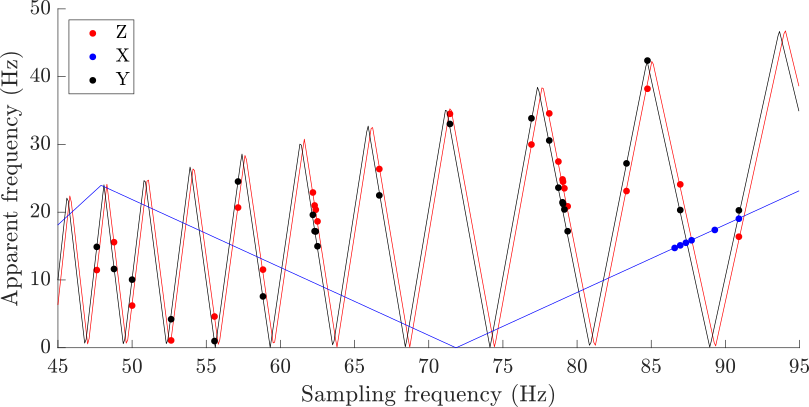
\includegraphics[width=\textwidth]{fig/tuneout/sawtooth_plot}
		\end{minipage}
		\hfill
		\begin{minipage}{0.3\textwidth}
		\vspace{0pt}
			\caption{Aliasing of the trap frequency oscillations under different sampling regimes. The sawtooth function is a one-parameter fit which determines the underlying frequency of the centre-of-mass oscillations.}
			\label{fig:sawtooth_plot}
		\end{minipage}
	\end{figure}	

	Figure \ref{fig:sawtooth_plot} shows the \emph{apparent} frequencies of oscillation in each axis as a function of sampling frequency, as measured using the pulsed atom laser method described above.
	The maximum sampling frequency is limited to about 100Hz by the temporal width of the BEC pulse landing on the detector. We fit the apparent oscillation frequency in each axis with the one-parameter model Eqn. \ref{eqn:Z_N}. We thus determine the characterisic frequencies of the magnetic trap to be $(\omega_x,\omega_y,\omega_z)= 2\pi\times(426.6(1),55.4(3),428.41(4))$ Hz \footnote{Values in brackets represent variation over many experiments.}.

	In fact, this measurement uses much more data than is strictly necessary to obtain $f$ unambiguously, and is presented to illustrate the technique. 
	One can obtain faster estimates by varying $f_s$ slightly and computing the gradient $df_a/df_s$ which unambiguously fixes $Z_n$ (assuming one does not accidentally cross a zone boundary, see eqn \ref{eqn:Z_N}).
	Therefore by selecting a sampling frequency near the middle of a known Nyquist zone, one can then monitor changes in the underlying frequency $f$ with single measurements (again, assuming the shift is not great enough to push the signal into a different Nyquist zone).
	We find that our trap frequency is extremely stable, and given the small perturbation of the probe beam, we ensure that the net oscillation frequency signal remains within a single Nyquist zone  over the entire data collection campaign. 
	Specifically, we determined that the oscillations in the \(y\)-axis are in the 5\textsuperscript{th} Nyquist zone when sampling at 125~Hz. The corresponding correction to obtain the underlying frequency from the aliased frequency is
	\begin{equation}
	    f_{\text{real}}=3 f_{\text{sampling}} + f_{\text{aliased}}.
	\end{equation}
	where \(f_{\text{real}}\) is the underlying frequency, \(f_{\text{aliased}}\) is the apparent frequency obtained from the fit, and \(f_{\text{sampling}}\) is the sampling frequency. 


	\begin{figure}[t]
	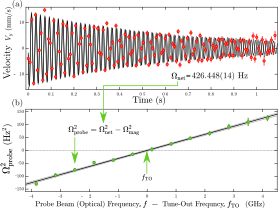
\includegraphics[width=\textwidth]{fig/tuneout/freq_measurement}
	\caption{
	Determining the tune-out frequency for fixed polarization. As discussed in the main text, fits to period samples of the trap motion (a) are used to obtain $\Omega_\textrm{probe}$ and thus find the point of null response.
	}
	\label{fig:freq_method} 
	\end{figure}


	\begin{figure*}
	\centering
	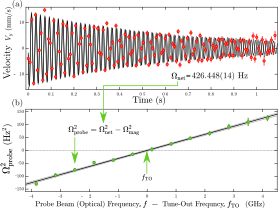
\includegraphics[width=0.8\textwidth]{fig/tuneout/freq_measurement}
	\caption{
	\todo{update Caption, } The mean velocity of each pulse in the \textit{x}-direction ($v_x$) is used to trace out the oscillation over time (red points) and extract the oscillation frequency with a dampened sine wave fit (solid line). A single experimental realization is shown. (C) The squared probe beam trap frequency (response) is found using a separate measurement of the magnetic trap frequency. This measurement is repeated over a small range of optical frequencies. The tune-out is extracted by finding the \textit{x}-intercept of the response as a function of probe beam frequency using a linear fit (black solid line). Light grey lines show the model \(1\sigma\) confidence intervals. All error bars represent the standard error in the mean.
	}
	\label{fig:exp_schematic} 
	\end{figure*}



\subsection{Polarization dependence of the tune-out}
	% summarise the stages of measurement
	\todo{Put polarization theory here and then explain the various stages of analysis.}

	To determine the tune-out frequency (\(f_{TO}\)) for a given polarization state of the probe beam (\( \mathcal{Q_{L}},\mathcal{V} \)), we find the probe beam (optical) frequency $f$ for which the measured probe beam trap frequency \(\Omega_{\text{probe}}^2\) is zero (using the methods described in section \ref{sec:trap_freq_measure} above). 
	This is done by measuring \(\Omega_{\text{probe}}^2\) as a function of the probe (optical) frequency in a small range about the tune-out frequency. 
	This range is chosen in order to minimize the nonlinearities that are present at large probe beam potentials while still presenting a sufficient signal-to-noise for interpolation of the the linear response. For the data presented here, we used scans out to 4.5~GHz either side of the tune-out.
	To perform these scans we change the set point of the probe beam (optical) frequency feedback system every two trap frequency measurements (after each set of one probe-on measurement and one calibration). We step through 13 frequency values over this 9~GHz range. We then use a linear fit to extract the probe beam frequency where \(\Omega_{\text{probe}}^2=0\), which corresponds to the tune-out frequency for this polarization.



	To measure \(f_{\mathrm{TO}}(-1,0)\) we perform three stages of measurements. Firstly, for a given probe beam polarization and (optical) frequency we make a measurement of the polarizability via the (spatial) oscillation frequency of ultracold helium in the combination of an optical dipole potential of the probe beam and the magnetic trap. 
	Secondly, we repeat many of these measurements while varying the probe beam (optical) frequency to find the optical frequency where the polarizability goes to zero (the tune-out frequency, \(f_{TO}(\mathcal{Q_A},\mathcal{V})\) ) for this probe beam polarization. 
	Finally, we repeat the second stage at many values of probe beam polarization in order to extract  \(f_{\mathrm{TO}}(-1,0)\), the tune-out for the particular light polarization (in the atomic frame) which we use to compare with theoretical predictions.

\subsection{Data Vetos}

	An experiment this complex is susceptible to many potential failure modes, and it is prudent for the experimentalist to mitigate against them.
	To ensure the integrity of the data set used for analysis we complemented the aforementioned control systems with a veto checklist in the data preprocessing pipeline.
	This consisted of a software screening procedure which discarded any measurements where any of the following essential conditions failed to hold. These conditions result in a loss of only one shot in $10^{4}$ across the whole dataset. 

	\textbf{Single-mode laser:}	On rare occasions we observed that the Ti:S laser would spontaneously run in a multi-mode regime (i.e. when multiple optical frequencies were resonant in the cavity and present in the output) which would cause the wavemeter to provide inaccurate frequency measurements. We eliminated runs where this happened by recording the output of a scanning Fabry-Perot cavity (Thorlabs SA200-5B). We scanned the cavity over twice its full free-spectral range in a sawtooth manner by scanning the voltage across a piezoelectric actuator, which modulates the cavity length, at frequency of 20 Hz. 
	We recorded the piezo and photodiode voltage during the interrogation and also in a $\sim0.2$~s period before and after.
	The multimode detection condition was triggerd when the separation between peaks detected in the photodiode voltage were less than the free-spectral range, indicating the presence of multiple optical frequencies.
	We used a peak detection threshold of $1.5\times10^{-3}$ of the peak transmission intensity to distinguish spurious peaks from electronic noise (all multimode conditions we  observed had peak intensities some orders of magnitude larger than this).

	\textbf{Stable probe power:}		We employ a check on the probe beam power as measured with the probe beam photodiode which measures the power of the beam just before it enters the experimental chamber, as shown in Fig.~\ref{fig:exp_diagram}. This ensures that the power feedback system is operating at set point in all measurements used in the analysis. Restrictive thresholds are set on the mean ($<0.02$ fractional difference to set point), standard deviation ($<0.05$ of set point) and maximum difference to set point ($<0.03$ of set point) of the power during interrogation.

	\textbf{Stable probe frequency:}		The probe beam frequency at each measurement is taken to be the average optical frequency returned by the wavemeter. Shots were rejected if the frequency records in the lock loop's log file has a standard deviation greater than $3$~MHz or a range greater than $5$~MHz.

	\textbf{High atom number:}		Shots with very low atom number would lead to inaccurate determinations of the trapping frequency because the damped-sine fit would not be able to fit to many points. We mitigated this by screening out shots with less than $2\times10^{5}$ detected atoms. We found that the choice of threshold introduces a negligible systematic shift in the final tune-out determination, hence we could use shots with a wide range of atom numbers (provided the fits converged).


\subsection{Fitting}
 
	To find \(f_{\mathrm{TO}}(-1,0)\) we measure the tune-out frequency and \(\mathcal{Q_{L}},\mathcal{V}\) over a range of $\lambda/2$, and $\lambda/4$ wave-plate angles (75 combinations used here) and then fit the above model [Eq.~(\ref{eqn:tune_out_eq})] to this set of \(\{\mathcal{Q_{L}},\, \mathcal{V},\, f_{TO}\}\) data using the free parameters $f^{S}_{TO}$,\, $\theta_{\mathcal{L}}$,\, $\theta_{k}$,\, $\beta^V$, and $\beta^T$ (see Fig.~\ref{fig:full_tune_out} for fit of full model with polarization data from pre and post vacuum chamber). This free fit is unable to fully constrain the free fit parameters, critically, giving equal agreement between either polarity of \( \beta^T \) and thus preventing a determination of \(f_{\mathrm{TO}}(-1,0)\). 
	To eliminate one of these cases, we introduce a constraint on the sign of  \( \beta^T \) using  measurements and simulations of the magnetic field pointing and theoretical atomic structure calculations, both of which agree with the sign constraint \( \beta^T >0 \).
	With this constraint added, we use an uncertainty-weighted fit to find \(f_{\mathrm{TO}}(-1,0)\) by evaluating the resulting model at \(\mathcal{Q_{A}}=-1,\mathcal{V}=0\). The statistical error in the calculated \(f_{\mathrm{TO}}(-1,0)\) is determined with a bootstrapping technique wherein the constrained fitting procedure is repeated on subsets of the data to estimate the uncertainty in the full fit \cite{bryce_bootstrap_error_code}. 
	Four of the fit terms ($\theta_{\mathcal{L}}$, $\theta_{k}$, $\beta^V$, and $\beta^T$) are interdependent (reflected in their nondiagonal covariance matrix) and therefore the result of this fit cannot be used to find these values without extra information (such as measuring all but one such parameter). However, this does not effect the prediction of \(f_{\mathrm{TO}}(-1,0)\).

	% \begin{figure}
	% \centering
	% 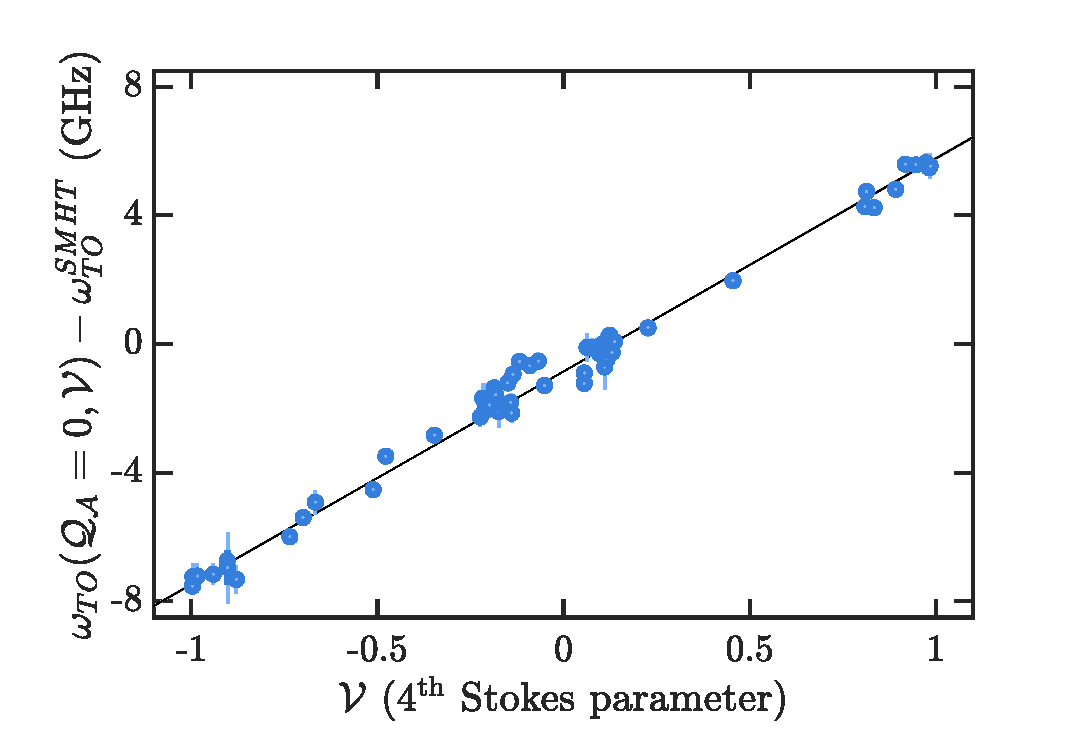
\includegraphics[width=8.6cm]{fig/tuneout/to_v_dependence.eps}
	% \caption{Dependence of the measured tune-out on $\mathcal{V}$ when projected to $\mathcal{Q}=0$ using the fit model. The light error bars represent the standard deviation in the tune-out measurements that make up each point, the thick blue error bar shows the standard error in the weighted mean (smaller than the marker of most points).
	% }
	% \end{figure}

	For display in Fig.~\ref{fig:full_tune_out} the $\mathcal{Q_{A}}$ value is calculated using the fit $\theta_{\mathcal{L}}$ and $\mathcal{Q_{L}}$ and the measured \(f_{TO}\) is displayed as a function of $\mathcal{Q_{A}}$, $\mathcal{V}$. In Fig.~\ref{fig:full_tune_out} we also display the tune-out calculated for polarization data sets taken before and after the vacuum chamber.%For display each polarization is combined, with the uncertainty weighted mean, standard error of the weighted mean  standard deviation.




	\begin{figure}
	\centering
	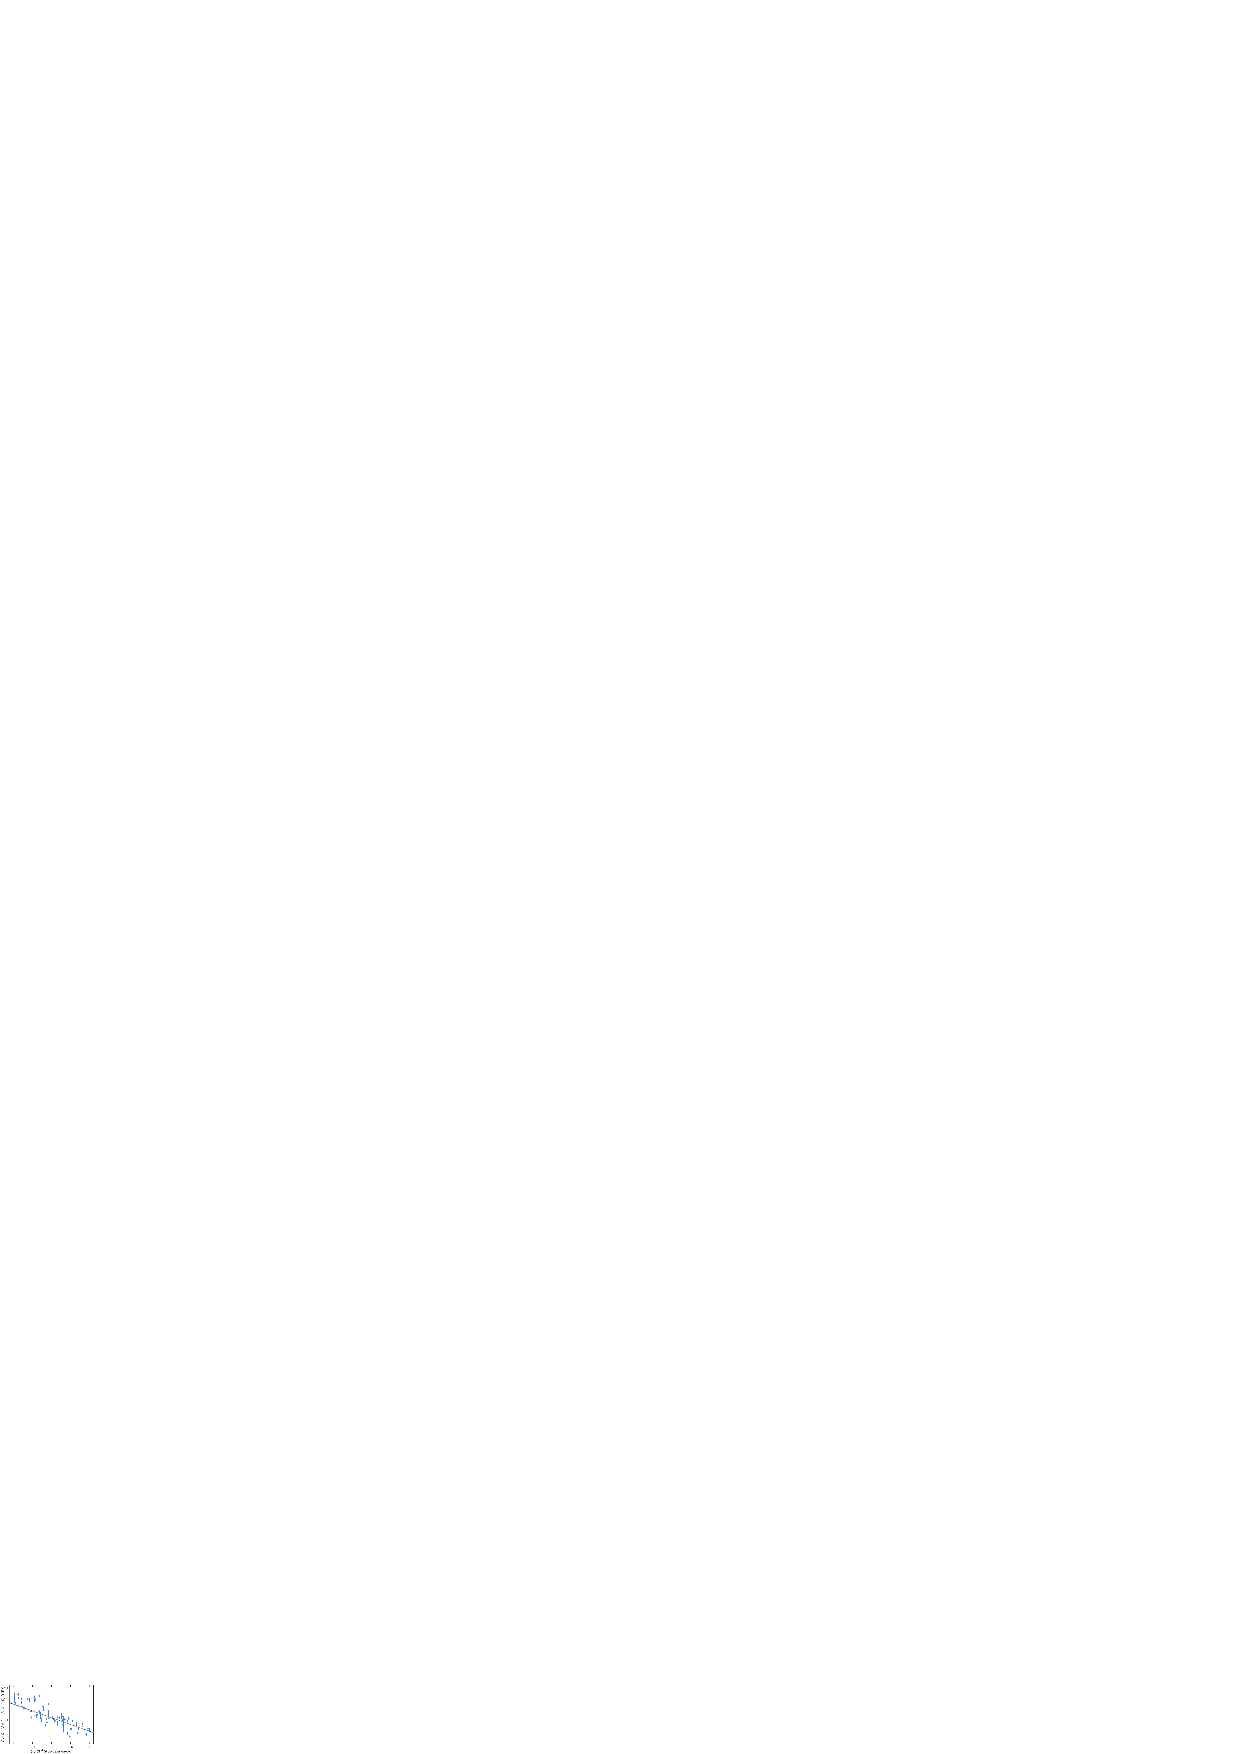
\includegraphics[width=\textwidth]{fig/tuneout/to_q_crop.png}
	\includegraphics[width=\textwidth]{fig/tuneout/to_v_crop.png}
	\caption{\textbf{Tune-out dependence on probe beam polarisation:}
	(A) Dependence of the measured tune-out on $\mathcal{Q_{A}}$ when interpolated to $\mathcal{V}=0$. (B) Dependence of the measured tune-out on $\mathcal{V}$ when interpolated to $\mathcal{Q_{A}}=-1$. The linear fits are both of the form of Eq.~(\ref{eq:TO_model}), with fit parameters \(f_{TO}(-1,0)=725\,736\,700\,(40)\)~MHz, \(\beta^V \cos(\theta_k)=13\,240\,(70)\)~MHz, \(\beta^T \sin^2(\theta_k)=1\,140\,(20)\)~MHz (uncertainties represent only statistical uncertainty; see Ref.~\cite{ArxivTO} for full error budget). Error bars show the estimated standard error.
	} 
	\label{fig:pol_TO} 
	\end{figure}


	% scraps
	%\href{https://github.com/spicydonkey/sewm}{sewm code} along with unweighted

	%It is clear here that the estimated statistical error in the determined TO frequency for each scan is far less than spread between the the model and the data. (factor of 6 between SEWM of combined data and the sd of redisulas, will calc for each unbinned data pt) We attribute this to imperfections in the polarization measurement and variation of the magnetic field pointing.

	%The fit is weighted by the square of the uncertainty in each TO measurement $1/\sigma^2_{f_{TO}}$. The measured TO for each xx shot scan over wavelength for a given polarization is included in the fit as its own data point.
	%The fit is conducted with a global least squares prefitter that is constrained such that $-\pi/4<\theta_k<\pi/4$ and  $\beta^T>0$ which is then fed to an unconstrained fitter. 
	%In this way only a single parameter is required from theory, namely the sign of the tensor polarizability around the TO wavelength. This approach assumes that the tensor and vector polarization is approximately constant about the TO, consistent with theory [REF]\brycecom{from LYT}.

	% the frequency (wavelength) of light at which the atoms experience no perturbation is determined for some input probe polarization state and (ii) many of these measurement's (with varying degrees of circularity and linear orientation) are  combined and fit in Stokes space to determine the TO Scalar Minus Half Tensor (TOSMHT). The analysis for a given polarization state generally consists of hundreds of runs of the experiment grouped together to produce a measured TO for that polarization configuration.

	%and permits us to discern a peak potential energy of as little as 10$^{-35}$J. This is, to our knowledge, the smallest precision in a potential energy measurement reported to date \cite{ArxivTO}.  


\section{Systematic effects}

	A summary of the systematic shifts is shown in \autoref{tab:results}. 
	The accuracy of this measurement of $\fto$ is limited by uncertainty in the polarization of the laser light. 
	Each contribution is described in more detail below. 

	\begin{table}[t]
	\centering
	% \begin{ruledtabular}
	\begin{tabular}{l|r|r}
	Term              & Estimate &  Uncertainty \\
	\hline
	Measured Value      & 725\,736\,810             & 40      \\
	Polarization        & & \\
	\, \, - Birefringence & -100                   & 200   \\
	\, \, - Beam Anisotropy & 0                   & 150   \\
	Method Linearity    & 24                   & 30       \\
	Hyperpolarizability           & -30                   & 50   \\
	Broadband Light     & 0                     & 30      \\
	DC Electric field   & 0                     & \(\ll 1\) \\
	Wave-meter          & 0                     & 4    \\
	\hline
	Total               &  725\,736\,700            &  260
	\end{tabular}
	% \end{ruledtabular}
	\caption{Contributions to measured tune-out frequency with associated systematic uncertainties (MHz). The measured value is found using only polarization data measured after the vacuum chamber. The polarization row gives the average of the tune-out frequencies calculated using polarization data pre and post vacuum chamber relative to the measured value, where the uncertainty is the discrepancy between these values. Note that uncertainties are added in quadrature.}
	\label{tab:results}
	\end{table}

\subsection{Polarization}

	 The extraction of \(\fto(-1,0)\) needs an accurate determination the probe beam polarization at the point of interaction with the atoms. 
	 As we did not have polarization optics mounted in vacuo, we inferred it from measurements outside the vacuum system. 
	 We estimated the contribution of two effects: the birefringence of the vacuum windows and the variation of polarization across the beam profile.
	 


\subsubsection{Birefringence}
	
	The polarization of the light may be altered as it passes through the final optical element: The glass window into the vacuum chamber.
	This means that the in-vacuum polarization may be different from the polarization set by the pre-insertion optics and measured prior to vacuum entry.
 	We estimated the size of this effect by measuring the probe beam polarization before it entered the vacuum system, and again after it exited through a second window\footnote{A portion of the probe beam escaped back through the LVIS and then the horizontal MOT window, making this possible.}.
 	We determined the error by running the $\fto(-1,0)$ analysis, as above, using both sets of polarization measurements (see Fig.~\ref{fig:full_tune_out}). 
 	We found that these values agreed within \(200\)~MHz, and hence used this as the uncertainty associated with the window birefringence. 

\subsubsection{Polarization across the beam}

	We also also observed a small variation in the polarization across the transverse profile of the beam.
	We determined that the mirrors in the pre-vacuum optics were the culprit.
	We characterized this by measuring polarization at several points across the beam.
	Using the polarization measured far from the beam axis produces a value of \(f_{\mathrm{TO}}(-1,0)\) that is up to \(400\)~MHz different from using the polarization at the beam center. 
	However, these contributions from differently-polarized light are weighted by their respective intensities, and accordingly the  weighted values produce a \(150\)~MHz uncertainty in $\fto$.

\subsection{Linearity} \label{sec:syst.subsec:lin}

	Our analysis to obtain \(f_{\mathrm{TO}}(-1,0)\) assumes the perturbation $\omega_\mathrm{probe}^2$ is linear with respect to the probe beam frequency. 
	This is only approximately true: The polarizability is a nonlinear function of laser frequency at larger distances from $\fto$ (on the THz scale). 
	Nonetheless, quadratic (and higher) terms included in the fits to the laser scans were not statistically different from zero.
	\rem{The polarizability $\alpha(f)$ about the tune-out is approximately linear in frequency. However, this is not exact. Using a model of the polarizability we find that fitting a linear dependence over 4~GHz either side of the tune-out results in a fit intercept which is $-88(1)$~kHz from the true tune-out. This shift would increase to $-9.6(2)$~MHz if measurements were taken 40~GHz about the tune-out. A quadratic fit reduces this shift to 0.6~kHz and 40~kHz in the 4~GHz and 40~GHz cases respectively.}

	Moreover, the relation $\Omega_{\text{net}}^2=\Omega_{\text{trap}}^2+\Omega_{\text{probe}}^2$ was derived assuming a harmonic potential, which ignores higher-order derivatives of the Gaussian optical potential.
	Again, this was not found to be significant.
	A characteristic feature of oscillatory motion in anharmonic potentials is that the period of oscillation depends on the total energy (\emph{i.e.} on the amplitude).
	We checked for this by fitting the damped-sine model to different (contiguous) subsets of the atom laser pulses.
	While we did observe that the largest oscillations were 0.3 Hz slower than the smallest, there was no significant effect on the zero crossing $\fto$.  


	\begin{figure}
	    \centering
	    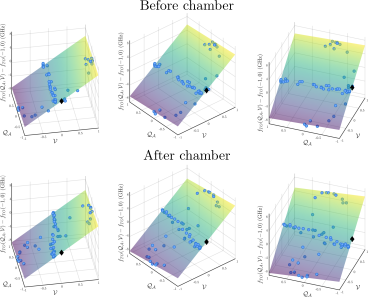
\includegraphics[width=\textwidth]{fig/tuneout/polz_pre_post}
	\caption{Visualizing the fit to $f_{TO}$ as a function of the polarization parameters $\mathcal{Q_{A}}$,\, $\mathcal{V}$  (see Eq.~(\ref{eqn:tune_out_eq})). The top row shows a fit using the polarization data taken before the vacuum chamber. The bottom row uses data taken after the vacuum chamber.  Each tuneout measurement is shown as a blue point. Note that (a-c) and (d-f) show, respectively, different viewing angles on the same data. The black diamond shows the value for \(f_{\mathrm{TO}}(-1,0)\) obtained in each case: \(f_{\mathrm{TO}}(-1,0)=725\, 736\, 810(40)\)~MHz in the top row, and \(f_{\mathrm{TO}}(-1,0)=725\, 736\, 610(40)\)~MHz in the bottom row. The other fit parameters are \(\beta^V \cos(\theta_k)=13240(70)\)~MHz, and \(\beta^T \sin^2(\theta_k)=1140(20)\)~MHz.}
	% top data:\(\beta^V \cos(\theta_k)=13240(70)\)~MHz, and \(\beta^T \sin^2(\theta_k)=1140(20)\)~MHz
	% bottom data: \(\beta^V \cos(\theta_k)=13012(100)\)~MHz, and \(\beta^T \sin^2(\theta_k)=550(100)\)~MHz
	\label{fig:full_tune_out}
	\end{figure}

\subsubsection{Method Linearity}
	
	We measured \(\Omega_{\mathrm{probe}}\) as a function of probe beam power, with the polarization and frequency fixed, to constrain any shift with respect to probe beam intensity. A second-degree polynomial was sufficient to describe the  response (see Fig.~\ref{fig:probe_beam_linearity}), and we deduce that the tune-out could be shifted by \(-24(30)\)~MHz.

		\begin{figure}
	    \begin{minipage}{0.6\textwidth}
	    \vspace{0pt}
	    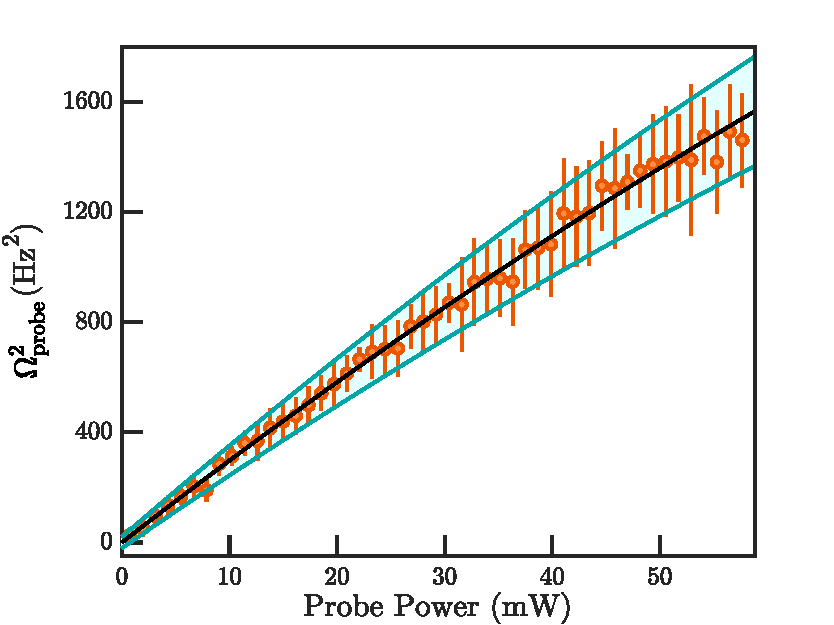
\includegraphics[width=\textwidth]{fig/tuneout/probe_beam_linearity}
	    \end{minipage}
	    \hfill
	    \begin{minipage}{0.4\textwidth}
	    \vspace{0pt}
	    \caption{Testing for nonlinear response versus power. We set the  probe frequency 20~GHz blue of $\fto$,  producing a strong potential, and fit the response against the power P (in watts) with the model \( \Omega_{\mathrm{probe}}^2 = a  P - b P^2 \).  The fit parameters are \(a=\text{30.3(1)}\times 10^{-3}\text{~Hz}^2\text{W}^{-1}\), \(b= \text{0.06(2)} \times 10^{-6}\text{~Hz}^2\text{W}^{-2}\). Higher-order terms  were not statistically significant. The \(1\sigma\) (observation) confidence interval is shaded. 	    }
	    \label{fig:probe_beam_linearity}
	    \end{minipage}
	\end{figure}



\subsection{Hyperpolarizability}

	The working above also assumes that the metastable-state energy shift due to a nonzero polarizability is a linear function of the light field intensity. 
	We combined theoretical predictions and experimental measurements to obtain an estimate for this error.
	

	\begin{figure}[t]
	    \centering
	    \includegraphics[width=\textwidth]{fig/tuneout/hyp_pol_v1}
	    \caption{Dependence of the tune-out on probe beam intensity. 
	    A linear fit returns estimates of the offset\(=725\,736\,090(50)\)~MHz and gradient\(=-1.2(1.5)\)~MHz/(Hz\(^2\)/GHz).
	    The shaded region shows the \(1\sigma\) observational confidence interval.
	    The rightmost point corresponds to a peak intensity of \(\sim4\times10^{8}\: \mathrm{W}\cdot \mathrm{m}^{-2}\). 
	    \todo{What was the intensity used in the experiment?}. 
	    The fit shows that any shift of the tune-out shift, with respect to the slope of the response is $30(50)$~MHz - statistically consistent with zero for the intensities used in the main measurement.
	    }
	    \label{fig:hyperpolarizability}
	\end{figure}

\subsubsection{DC Electric Field}

	A worst-case estimate of any DC electric field background is $2~\text{kV}\cdot\text{m}^{-1}$. 
	We can use an approach similar to that of the hyperpolarizability  and find a worst-case shift of \(10^{-2}\)~MHz.

\subsubsection{Theoretical treatment}

	The energy of an atom in the presence of an electric field \(E\) oscillating at a frequency \(f\) is 
	\begin{equation}
	\mathcal{E}=\mathcal{E}_0 - \frac{1}{2} \alpha(f) E^2 - \frac{1}{24} \gamma(f) E^4 + \ldots \, , \label{eqn:energy_shift}
	\end{equation}
	where \(\mathcal{E}_0\) is the energy of the unperturbed atom, \(\alpha(f)\) is the dynamic polarizability, and \(\gamma(f)\) is the (second) hyperpolarizability.  
	For a monochromatic light field, the time-averaged electric field amplitude is related to the intensity $I$ via
	\begin{equation}
	    E^2=\frac{2 I}{c \epsilon_0},
	\end{equation}
	where \(c\) is the speed of light and \(\epsilon_0\) is the permittivity of free space. 
	A tune-out measurement may be shifted due to the dynamic polarizability cancelling any contriburion from the hyperpolarizability. 
	We can estimate this shift by noting that, by definition, \(\mathcal{E}=\mathcal{E}_0\) at the measured tune-out, and expanding the polarizability to first order about the tune-out.
	Thus Eq.~(\ref{eqn:energy_shift}) gives 
	
	\begin{equation}
	 (f-f_\mathrm{TO} ) = - \frac{1}{12} \gamma(f) \left(\frac{2 I}{c \epsilon_0}\right) \left(1\left/ \frac{\partial\alpha}{\partial f}\bigg|_{f=f_\mathrm{TO}} \right. \right).
	\end{equation}
	From the theoretical calculations, the dynamic hyperpolarizability  is $6.964\times10^{-58}$ $\mathrm{C}^4\mathrm{m}^4\mathrm{J}^{-3}$ (about $-1.12\times10^{7}$ a.u.) at the tune-out. The probe beam intensity in the experiment was less than $10^{9}\: \mathrm{W} \mathrm{m}^{-2}$ and thus a shift due to the hyperpolarizability is  constrained to be below 1.5~MHz, which is dominated by other systematic effects.

	\com{High precision atomic theory has shown that the dynamic hyperpolarizability at the tune-out is \(6.964\times10^{-58}\: \mathrm{C}^4\mathrm{m}^4\mathrm{J}^{-3}\) ($-1.117\times10^{7}$ atomic second hyperpolarizability units), this is substantially more than predictions elsewhere \cite{Grunefeld} \(1.2\times10^{-58}\: \mathrm{C}^4\mathrm{m}^4\mathrm{J}^{-3}\) ($-2\times10^{6}$ atomic second hyperpolarizability units).
	Taking the larger value we find the intensity dependent shift is  $2\times10^{-3}\: \mathrm{Hz} \mathrm{W}^{-1} \mathrm{m}^2$. For the probe beam intensities used in this experiment ($<10^{9}\: \mathrm{W} \mathrm{m}^{-2}$) the magnitude of this shift is $<1.5$~MHz, well below other systematic errors.}

\subsubsection{Experimental treatment}

	We also made constrained the effect of the hyperpolarizability using an independent experimental approach, by studying the effect of the light intensity on the the measured tune-out. 
	The gradient of \(\Omega_{\text{probe}}^2\) with respect to the laser frequency gives an indirect measurement of the intensity in the region of interaction. 
	We measured the tune-out as a function of probe beam intensity (see Fig.~\ref{fig:hyperpolarizability}) and found that the effect was consistent with zero.

\subsection{Broadband Light}
	\todo{Integral expression}

	Broadband background light could be produced, for example, by  spontaneous emission in the Ti:S laser which is then amplified in the laser cavity. 
	In the presence of weak broadband light, the energy of the atom shifts by the (integrated) pointwise product of the spectral power density and the polarizability. 
	Because the magnitude of the polarizability increases superlinearly with the detuning from the tune-out, this effect puts a large weight on the tails of the laser line and may shift the apparent tune-out from its actual value. 
	This places demanding constraints on the tolerable spectral background of the probe laser. 
	This has been a challenge for measurements in other species \cite{HolmgrenThesis}. 
	
	Our use of a frequency doubled laser system provides some protection from this because the doubling cavity suppresses light resonant in the Ti:S. 
	Futher suppression is obtained by passing the probe beam through a series of optical filters: a 450~nm shortpass filter (Thorlabs FESH0450, optical density $>5$ between 450~nm and 1200~nm), a 415~nm band-pass filter (Semrock FF01-415/10-25, with a 27~THZ (15.3~nm) FWHM and optical density $>4$ between 250-399~nm and 431-1100~nm), and finally an angle-tunable filter with a 0.9~THz (0.5~nm) FWHM, which we centred on \(\sim 413\)~nm.

	In principle, one could use a spectrometer to measure the spectral power density of the background, but the requisite dynamic range to observe such small effects near a laser peak makes this unfeasible.
	Instead we use scheme similar the one described in \cite{Leonard15}, and measure the tune-out as a function of the number of (progressively narrowing) filtering stages.
	We can then estimate the shift in the  final measurement. 
	As shown in Fig.~\ref{fig:broadband light dependence},  the measured tune-out frequency is independent of number of filters (within statistical error). 
	Therefore we take the standard deviation between the various filters (\(30\)~MHz)  as the uncertainty associated with the spectral background.
	 
	\begin{figure}[t]
	    \centering
	    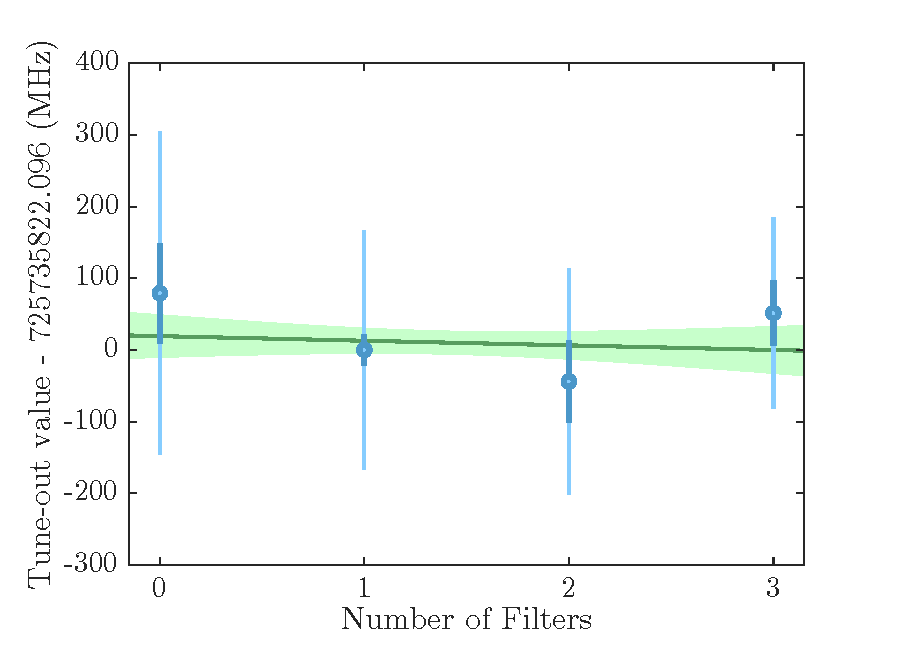
\includegraphics[width=\textwidth]{fig/tuneout/filt_dep}
	    \caption{The tune-out frequency as measured with fixed probe beam polarization and power, as a function of the number of filters in the beam path. The gradient of this dependence is \(-4.24(12)\)~MHz/filter, and hence zero within error.\rem{4(12) or 4.24(0.12)?}
	    }
	    \label{fig:broadband light dependence}
	\end{figure}



\subsection{Magnetic Field Pointing}
	
	Although we do not need perfect knowledge of the magnetic field orientation to employ the preceding method, the field pointing could drift durnig the months-long data acquisition period, and thus presents a potential source of systematic error.
	To constrain this effect, we simulated the magnetic trap \cite{Dall07_laser} and field stabilization system \cite{Dedman07} used in these experiments \footnote{The source code is available at \cite{mag_trap_simulator}.}.
	Such a systematic shift can divided into two contributions: the short-time variation in field pointing due to an atom's motion within the trap during the interrogation, and any long-term drift due to imperfections in the field control system.
	In the trap configurations used in this experiment, the magnetic field at the trap centre subtends a  $5.9 \circ $ angle relative to the long axis of the chamber, with which the probe beam is aligned, and a $0.019 \degree$ angle relative to the horizontal plane. 
	\com{The simulations show that the polar angle of the magnetic pointing, relative to the y axis, is $0.019 + 0.88 s \degree$ where s is the displacement }

\section{Discussion}
	\todo{Not quite sure what this para is saying specifically. Don't rephrase, rewrite.}
	Figure~\ref{fig:contributions} shows a comparison of contributions to the theoretical value of the tune-out and the uncertainties in both the experimental and theoretical determination.
	The theoretical and experimental uncertainties in combination yield a  \(\sigma{\sim} 260\)~MHz) are able to discern the contribution of QED effects (\({\sim} 30 \sigma\)), and are similar to the retardation corrections to the dipole interaction (\({\sim} 2 \sigma\)), but much greater than the contribution of finite nuclear size effects (\(5\)~MHz). 
	We show a comparison of our experimental and theoretical uncertainties to the main contributions of interest to the theoretical value in 
	 
	\begin{figure}[t]
	    \centering
	    \includegraphics[width=\textwidth]{fig/tuneout/contribution_bar_chart_v7.png}
	    \caption{Theoretical contributions to the tune-out value in comparison to uncertainties in the theoretical and experimental determinations of the \(\TO\) tune-out frequency.}
	    \label{fig:contributions}
	\end{figure}

	This is the first measurement which has sufficint precision to probe  the retardation corrections which are typically omtted when calculating the frequency-dependent polarizability \cite{Drake19, Pachucki19}. 
	As a result we find a \({\sim} 2.5 \sigma\) difference between experiment and theory, including an estimate of the uncertainty due to terms excluded from the theoretical calculation.  
	Notably, if we ignore the retardation correction (as proposed in Ref.~\cite{Pachucki19} and implemented in tune-out frequency calculations for the first time in this work), then the difference is only \({\sim} 0.5 \sigma\).  
	If the precision of the measurement were to be  improved by an order of magnitude, the effect of the retardation contribution could be subject to a more stringent test.


\subsection{Precision measurements of potential energy}
	\todo{Rework after analysis}

	A single scan takes approximately 700~s (12~minutes) and consists of 26 trap frequency measurements (BEC productions). We typically achieve an uncertainty in the tune-out of approximately 1.2~$\text{GHz}/\sqrt{N_\text{shots}}$, where \(N_\text{shots}\) refer to the number of BEC's used (either calibration or probe beam measurements). For example, 26 trap frequency measurements (one full scan) gives an uncertainty of $\sim 1.2\;\mathrm{GHz}/\sqrt{26}=235$~MHz. The number of measurements taken to find the tune-out for a given polarization varies from 50 to a few thousand for the data presented here.

	Using this method we can infer the peak value of the energy shift imparted by the probe beam onto the atoms. Through Eq.~(\ref{eq:omega_from_u}), a measurement of the probe-induced shift in trap frequency determines the curvature of peak of the Gaussian optical potential energy surface. Along with a measurement of the beam profile at the focus, the inferred curvature completely specifies the geometry of the optical potential. Thus, we can indirectly measure the absolute energy shift in the $\MetastableState$ state with a sensitivity of $1.7\cdot10^{-33}\mathrm{J}/\sqrt{\mathrm{sec}}$, where the time is the probe beam interrogation time. In the case of the probe beam polarization with the lowest frequency uncertainty in $f_\textrm{TO}$, (30~MHz), the minimum potential energy peak we can thus discern with is approximately $10^{-35}\mathrm{J}$ ($U/k_B=3$~pK).

\subsection{Comparison With Previous Oscillator Strength Ratio Measurements}
	\todo{Rework or omit with reference}
	We claim that this measurement of the $\TO$ tune-out wavelength represents the most precise measurement of transition rate ratios made to date in an atomic system. To find the uncertainty in the ratio of oscillator strengths we start by generalizing the treatment given in Ref.~\cite{Mitroy13} by using a model of the polarizability of a three level system.
	\begin{equation}
	\alpha(f) = \frac{\mathfrak{F}_1}{E_1^2-h^2 f^2}+\frac{\mathfrak{F}_2}{E_2^2-h^2 f^2}
	\end{equation}
	where $\mathfrak{F}_1$, $\mathfrak{F}_2$ correspond to the oscillator strengths, and $E_1$, $E_2$ the excitation energy of the respective transitions, $f$ is the photon frequency, and \(h\) is Planck's constant. 

	% In this simple model the tune-out is given by
	% \begin{equation}
	%     f_{TO}=\frac{\sqrt{E_{1}^2 \mathfrak{F}_2+E_{2}^2 \mathfrak{F}_1}}{h \sqrt{\mathfrak{F}_1+\mathfrak{F}_2}} .
	% \end{equation}
	If we introduce  the ratio of the oscillator strengths $X=\mathfrak{F}_2^2/\mathfrak{F}_1^2$ and note that by definition \(\alpha(f_{TO})=0\), substituting in the above expression and solving for this ratio we find
	\begin{equation}
	    X =\frac{ (E_2^2 -h^2 f_{TO}^2 )^2}{(E_1^2-h^2 f_{TO}^2)^2}.
	\end{equation}
	We can hence find the sensitivity of the value of \(X\) to changes in the tune-out frequency.
	% \begin{equation}
	%     \frac{\partial f_{to}}{\partial X} = \frac{(E_1-E_2) (E_1+E_2)}{4 h (1+\sqrt{X})^{3/2} \sqrt{E_2^2 + E_1^2 \sqrt{X}}}
	% \end{equation}
	% And then give the fractional uncertainty in the derived transition strength ratio.
	\begin{equation}
	    \frac{\delta X}{X} = \frac{\partial X} {\partial f_{TO}} \frac{1}{X} \cdot \delta f_{TO} =
	    \frac{2  h^2 f_{TO} (E_1^2-E_2^2)}
	    {(E_1^2-h^2 f_{TO}^2) (-E_2^2 + h^2 f_{TO}^2 )} \cdot \delta  f_{TO} = \frac{-2 f_{TO}^2 (f_1^2-f_2^2)}{(f_1^2-f_{TO}^2)(f_2^2-f_{TO}^2)} \frac{\delta  f_{TO}}{f_{TO}}
	\end{equation}
	where \(E_1=h f_1\) and \(E_2=h f_2\).
	To evaluate other work in the literature we use the frequency of the dominant transitions and the measured tune-out value to then derive the estimated sensitivity to the ratio of transition strengths. This method is approximate and neglects the contribution from the DC polarizability, however this is a small effect and not needed for such coarse comparison of sensitivity. Given the dominant transition manifolds at 276.7465~THz (\(\MetastableState \to \TOUpperStateManifold \)) and 770.7298~THz (\(\MetastableState \to \TOLowerStateManifold\)), as well as our value for the tune-out frequency of \(f_{TO}=725.7367\)~THz, we reach a fractional uncertainty in the oscillator strength ratio of 6~ppm, an improvement on the previous record of 15~ppm set by Ref.~\cite{Leonard15}. We note that the fractional uncertainty in the ratio of oscillator strengths is identical to the fractional uncertainty in the ratio of transition matrix elements which are calculated in Ref.~\cite{Leonard15}.

\subsection{Conclusion}

	To summarise, our experimental determination of 725\,736\,700\,$(40_{\mathrm{stat}},260_{\mathrm{syst}})$ MHz is a \(20\)-fold improvement over the first experimental determination, and is 2.5$\sigma$ larger than the theoretical prediction. 
	Our measurement has a relative precision better than $4\times 10^{-7}$, and constitutes the most precise measurement of transition rate information ever made in helium \cite{Mitroy13}
	Our measurement corresponds to a relative precision in oscillator strength ratio of 6 ppm \cite{ArxivTO}, which is a factor of two improvement on the previous record \cite{Mitroy13}. 
	Furthermore, our novel method for measuring the dipole potential is able to discern a peak potential energy of as little as 10$^{-35}$J. This is, to our knowledge, the smallest precision in a potential energy measurement reported to date \cite{ArxivTO}.
	 
	In future precision measurements of tune-out points, significant improvements would follow from more precise calibration of the light polarization.
	One solution would be to use in-vacuum optics and make finer measurements of the angle of the beam axis relative to the magnetic field.
	These improvements would allow for independent tests of the scalar, vector, and tensor polarizabilities, thus yielding more information about the structure of the helium atom and QED itself.

	The method above could be used to measure other tune-out frequencies in helium or other species.
	It could also serve as a means to investigate other issues relating to QED. 
	If a future measurement could be made with MHz-level precision,  this tune-out could be used to calculate the nuclear charge radius of helium. 
	Thus this method, and its future improvements, may continue to  clarify the `jewel of physics.'

\section{Note stash}

\subsubsection{Theoretical Basis of method}
	To measure the tune-out we must first be able to be measure the (real part of the) optical polarizability (\(\operatorname{Re}(\alpha)\)) at some given probe beam (optical) frequency. As only the null of this signal is used, absolute calibration is not required. However, the measurement should be linear to allow for linear interpolation of the polarizability as a function of frequency to find the tune-out.  A nonzero polarizability manifests as an optical dipole potential (\(U_{\mathrm{dip}}\)) in proportion to the intensity of the optical field (\(I\)) as \cite{Grimm00},
	 \begin{align}
	    U_{\mathrm{dip}}=-\frac{1}{2 \epsilon_{0} c} \operatorname{Re}(\alpha) I ,
	\end{align}
	where \(c\) is the speed of light, \(\epsilon_{0}\) is the vacuum permittivity, and \(\alpha\) is the complex polarizability. In this work, we detect the optical dipole potential through a modification to the (spatial) oscillation frequency of ultracold atoms confined in a harmonic magnetic trap when a Gaussian probe beam (oriented along the y axis) is overlapped with the trap minimum. The combined potential is given as
	 \begin{align}
	    U_{\mathrm{net}}& =-\frac{1}{2 \epsilon_{0} c} \operatorname{Re}(\alpha) 
	    \bigg[ 
	        \frac{2 P}{\pi w_0^2} \left(\frac{w_0}{w(y)}\right)^2 \exp\left( \frac{-2 (x^2+z^2)}{w(y)^2} \right)
	    \bigg]
	    + \frac{1}{2} m (x^2 \Omega_{\text{trap},x}^2  +y^2 \Omega_{\text{trap},y}^2  +z^2 \Omega_{\text{trap},z}^2 ), \label{eqn:net_U}
	 \end{align}
	where \(w(y) = w_0 \sqrt{1+\left( \frac{y}{y_R} \right)^2 }\) is the probe beam waist along the axis of propagation, \(w_0\) is the probe beam waist at the focus, \(y_R\) is the Rayleigh length, \(P\) is the total power of the beam and \( \Omega_{\text{trap},(x,y,z)} \) are the magnetic trap frequencies in the \((x,y,z)\) axes.
	To find the net trap frequency we use the expression   
	\begin{equation}
	\Omega=\frac{1}{2\pi\sqrt{m}} \sqrt{\frac{\partial^{2} U}{\partial x^{2}} \biggr\rvert_{\frac{\partial U}{\partial x}=0}}
	\label{eq:omega_from_u}
	\end{equation}
	for the trap frequency about a local minimum, where \(m\) is the mass of the oscillating particle, and apply it to the net potential in the \(x\)-axis. Applying Eq.~(\ref{eq:omega_from_u}) to Eq.~(\ref{eqn:net_U}) we obtain the net oscillation frequency as
	\begin{align}
	\Omega_{\text{net}}^2  & = \frac{1}{4\pi^2m} \frac{1}{2\epsilon_{0} c} Re(\alpha) \frac{2 P}{\pi w_0^2} \frac{4}{w_{0}^{2}} 
	+  \Omega_{\text{trap},x}^2,
	\end{align}
	which can also be expressed as the components from each potential source,
	\begin{align}
	\Omega_{\text{net}} & =\sqrt{\Omega_{\text{probe}}^{2}+\Omega_{\text{trap},x}^{2}}, \; \; \text{where }\\
	\Omega_{\text{probe}}& = \frac{1}{2\pi} \sqrt{\frac{1}{2m \epsilon_{0} c} Re(\alpha) \frac{2 P}{\pi w_0^2} \frac{4}{w_{0}^{2}}} \;.
	\end{align}
	Here \( \Omega_{\text{probe}} \) represents the spatial oscillation frequency of the probe beam by itself, which becomes imaginary when the trap is repulsive.
	Finally we see that a measurement of \( \Omega_{\text{probe}}^2 \) is linearly proportional to the real part of the polarizability. The treatment above is equivalent to a second order Taylor expansion about the trap minimum and provides a good approximation of the behaviour when the oscillation amplitude is small compared to the probe beam waist and when the probe trap frequency is small. For a discussion of the nonlinear effects see section \ref{sec:syst.subsec:lin} below.

\subsubsection{Dynamic Polarizability of Atoms in an Arbitrary light field}
	
	\todo{Substantially rewrite this section in own voice in own framework. Finally put the math togther as you worked on before. Separate the polarization theory from the polarizability theory. }

	Consider the interaction between an atom (in an external magnetic field \textbf{B} and Zeeman sublevel \(\ket{JM}\)) and a monochromatic classical light field given 
	\begin{align}
	    \textbf{E} &= \frac{1}{2} \mathcal{E} \textbf{u} e^{-i \omega t} \, + \, \text{c.c.},
	\end{align}
	where \(\omega\) is the angular frequency, \(\mathcal{E}\) is the electric field amplitude, and \textbf{u} the complex polarization vector. Note that only the real component of \textbf{E} has a physical meaning. For a strong enough magentic field (specifically when the off-diagonal terms are much smaller than the   Zeeman splitting of the sublevel, see \cite{} for more detail) the dynamic polarizability of the atom is:
	\begin{align}
	    \alpha(\omega) &= \alpha^s(\omega) + C \alpha^v(\omega) \frac{M}{2J} + D \alpha^T(\omega) \frac{3M^2-J(J+1)}{2J(2J-1)}
	\end{align}
	where \(\alpha^s\), \(\alpha^v\), and \(\alpha^T\) are the conventional scalar, vector, and tensor polarizabilities respectively. If we assume that the B-field is pointing along the \textit{z}-axis then the Coefficents \(C\) and \(D\) are given by:
	\begin{align}
	    C &= 2 \text{Im}(u_x^* u_y),\\
	    D &= 3|u_z|^2 -1
	\end{align}
	We can furthermore define these constants in terms of experimentally measurable variables (see ... for derivations)
	\begin{align}
	     C &= - \mathcal{V} \cos \left( \theta_k \right), \label{eqn:C} \\
	     D &= 3 \sin^2\left( \theta_k \right) \left(\frac{1}{2} +  \frac{\mathcal{Q}}{2}\right) -1 = 3 \sin^2\left( \theta_k \right) \left( \frac{1}{2} + \frac{1}{2} \frac{p_{max}-p_{min}}{p_{max}+p_{min}} \cos(2\theta_\varepsilon)\right) - 1 = 3 \sin^2(\theta_k) \mathcal{P}-1 \label{eqn:D}
	\end{align}
	where \(\mathcal{V}\) is the fourth stokes parameter, whose magnitude is given by \(|\mathcal{V}| = \frac{2\sqrt{p_{min}p_{max}}}{p_{min}+p_{max}}\) and sign depends on the handedness of the light, \(\mathcal{Q}=\frac{p_{max}-p_{min}}{p_{max}+p_{min}} \cos(2\theta_\varepsilon)\) is the second stokes parameter, and $\cos(\theta_\epsilon)=\text{Re}\left\{\textbf{u}\right\}\cdot(\textbf{B}\times \hat{k})$.

	Near the tune-out the the dynamic \(\alpha(\omega)\) and scalar \(\alpha^s(\omega)\) terms can be approximated by their truncate linear Taylor expansions about their respective zero points (\(\omega_{to}\), \(\omega_{s,0}\)):
	\begin{align}
	    \alpha(\omega) &= \alpha(\omega_{to}) + \difn{\alpha(\omega)}{\omega}{{}}(\omega-\omega_{to})=\difn{\alpha(\omega)}{\omega}{{}}(\omega-\omega_{to}), \\
	    \alpha^s(\omega) &= \alpha^s(\omega_{s,0}) + \difn{\alpha^s(\omega)}{\omega}{{}}(\omega-\omega_{s,0})= \difn{\alpha^s(\omega)}{\omega}{{}}(\omega-\omega_{s,0})
	\end{align}
	where \(\omega_{to}\) is the desired term. Note that for these approximations to be valid we need to only consider a small range about the respective zero values (\(\omega_{to}\), \(\omega_{s,0}\)), and as a consequence of this we must assume that the difference between these values is small. Substituting we obtain:
	\begin{align}
	    \difn{\alpha(\omega)}{\omega}{{}}(\omega-\omega_{to}) &= \difn{\alpha^s(\omega)}{\omega}{{}}(\omega-\omega_{s,0}) + C \alpha^v(\omega) \frac{M}{2J} + D \alpha^T(\omega) \frac{3M^2-J(J+1)}{2J(2J-1)}
	\end{align}
	The major contribution to the rate of change of the dynamic polarizability (\(\difn{\alpha(\omega)}{\omega}{{}}\)) is from the scalar polarizability (or equivalently that the vector and tensor terms are approximately constant over the range being considered), hence \(\difn{\alpha(\omega)}{\omega}{{}} \simeq \difn{\alpha^s(\omega)}{\omega}{{}}\). Rearranging and making this approximation into equation \ref{} we obtain:
	\begin{align}
	    \omega_{to} &= \omega_{s,0} - C \omega^v \frac{M}{2J} - D \omega^T \frac{3M^2-J(J+1)}{2J(2J-1)},
	\end{align}
	where \(\omega^{v,T} = \alpha^{s,T}/\difn{\alpha(\omega)}{\omega}{{}}\) are constants from the vector and tensor contributions. We are interested in the \(2^3S_1\) state \(\ket{J=1,M=1}\)
	\begin{align}
	    \omega_{to} &= \omega_{s,0} - C \omega^v \frac{1}{2} - D \omega^T \frac{1}{2},\\
	    &= \omega_{s,0} + \frac{1}{2} \omega^T + \frac{1}{2} \mathcal{V} \cos \left( \theta_k \right) \omega^v - \frac{3}{2} \mathcal{P} \sin^2(\theta_k) \omega^T.
	\end{align}
	If we set \(\mathcal{V}=0\) and \(\mathcal{P}=0\) we obtain \(\omega_{to} = \omega_{s,0} + \frac{1}{2} \omega^T\) which is the tune-out frequency for the dynamic polarizability \(\alpha(\omega) = \alpha^s(\omega) - \frac{1}{2}  \alpha^T(\omega)\).

	The dynamic atomic polarizability consists of the frequency dependent scalar, vector, and tensor components (\(\alpha^S(f),\alpha^V(f),\alpha^T(f)\) respectively). The total polarizability (and hence the tune-out) also depends on the degree of linear and circular polarization in the atom's reference frame, given by the second and fourth Stokes parameters \(\mathcal{Q_{A}}\) and  \(\mathcal{V}\) respectively, and on the angle $\theta_k$ between the laser propagation direction and the magnetic field vector \cite{LeKien13}. The tune-out frequency for the \(\MetastableState\) state and arbitrary polarization is: 

	% \begin{widetext}
	    \begin{equation}
	    f_{\mathrm{TO}}(\mathcal{Q_{A}}, \mathcal{V}) = f^{S}_{\mathrm{TO}} + \frac{1}{2} \beta^V \cos \left( \theta_k \right) \mathcal{V}  - \frac{1}{2} \beta^T \left[3 \sin^2\left( \theta_k \right) \left(\frac{1}{2} +  \frac{\mathcal{Q_{A}(Q_{L},\theta_{L}})}{2}\right) -1 \right],
	    \label{eq:TO_model}
	    \end{equation}
	% \end{widetext}
	where \(f^{S}_{\mathrm{TO}}\) is the tune-out frequency for the scalar polarizability $\alpha^S(f)$, \(\mathcal{Q_{A}(Q_{L},\theta_{L}})\) is the second Stokes parameter in terms of the laboratory measurement of the second Stokes parameter \(\mathcal{Q_L}\), and the angle between the lab and atomic frames \(\mathcal{\theta_{L}}\). Here, \( \beta^V\) and  \(\beta^T\) are the vector and tensor polarizabilities divided by the gradient of the scalar polarizability (with respect to frequency) at the tune-out \cite{ArxivTO}.


	We measure the tune-out \(f_{\mathrm{TO}}(-1,0)\), corresponding to a linearly polarised light-field whose polarisation axis is perpendicular to both the laser propagation and the magnetic field. For this configuration, the sensitivity to \(\theta_{k}\) and \(\theta_\mathcal{L}\) is minimized and the atomic polarizability simplifies to

	\begin{equation}
	    \alpha(f) = \alpha^S(f) - \frac{1}{2} \alpha^T(f). 
	    \label{eq:polarizability_2}
	\end{equation}

	We measure \(f_{\mathrm{TO}}(\mathcal{Q_{A}}, \mathcal{V}) \) as a function of the probe beam polarization parameters \(\mathcal{Q_{A}}\) and \(\mathcal{V}\) and interpolate using Eq.~(\ref{eq:TO_model}) to determine \(f_{\mathrm{TO}}(-1,0)\) (see Fig.~\ref{fig:pol_TO}). We take the sign of \(\beta^T\) from theory, but use no other predictions in our calculation. Thus, we determine a value of  725\,736\,700\,$(40_{\mathrm{stat}},260_{\mathrm{syst}})$ MHz for the \(f_{\mathrm{TO}}(-1,0)\) tune-out, including systematic effects \cite{ArxivTO}.

\subsubsection*{Calculation of \(C\) and \(D\)}
	Consider light propagating along the \(z-\)axis (\textit{i.e.} light vector \(\vec{k} = \left(0,0,1\right)\)), the Jone's vector of this light is given by:
	\begin{align}
	    \vec{u} &= \begin{pmatrix}
	    u_{0,x} \\
	    u_{0,y} e^{i \phi_y} \\
	    0
	\end{pmatrix}.
	\end{align}
	By definition the stokes parameters are defined as follows (in order from first to fourth):
	\begin{align}
	    \mathcal{I} &= |u_x|^2 + |u_y|^2 \\ 
	    \mathcal{Q} &= |u_x|^2 - |u_y|^2 \\
	    \mathcal{U} &= 2 \text{Re} \left(u_x u_y^*\right) \\
	    \mathcal{V} &= -2 \text{Im}\left(u_x u_y^*\right)
	\end{align}
	where \(\vec{u} = (u_x,u_y,u_z)\). Note we only wish to consider that normalised Jones vector/ Stokes parameters, hence \(\mathcal{I}=1=u_{0,x}^2+u_{0,y}^2\). Let the plane formed by the light vector \(\vec{k}\) and the magnetic field vector at the atoms (the quantization axis) \(\vec{b}\) be the \(y-z\) plane, hence if the angle between the light vector and the magnetic field is \(\theta_k\) then:
	\begin{align}
	        \vec{b} &= \begin{pmatrix}
	    0 \\
	    \sin(\theta_k) \\
	    \cos(\theta_k)
	\end{pmatrix}.
	\end{align}
	Now if the polarisation is rotated by an angle \(\theta_\varepsilon\) the Jone's vector becomes 
	\begin{align}
	    \vec{u} &= \begin{pmatrix}
	    \cos(\theta_\varepsilon) u_{0,x} -\sin(\theta_\varepsilon) u_{0,y} e^{i \phi_y}\\
	    \sin(\theta_\varepsilon) u_{0,x} +\cos(\theta_\varepsilon) u_{0,y} e^{i \phi_y} \\
	    0
	\end{pmatrix}.
	\end{align}
	Now to align with equations \ref{eqn:C} and \ref{eqn:D} we want to rotate the axes such that the B-field is pointing along the \(z\)-axis, this corresponds to a rotation matrix of:
	\begin{align}
	    R_k &= \begin{pmatrix}
	 1& 0 & 0 \\
	 0 & \cos(\theta_k) & -\sin(\theta_k) \\
	 0 & \sin(\theta_k) & \cos(\theta_k)
	\end{pmatrix}.
	\end{align}
	applying this we get the Jone's vector in the B-field's frame of reference (denoted \(\vec{u}'= R_k \vec{u}\) as
	\begin{align}
	    \vec{u}' &= \begin{pmatrix}
	    \cos(\theta_\varepsilon) u_{0,x} -\sin(\theta_\varepsilon) u_{0,y} e^{i \phi_y}\\
	    \cos(\theta_k) \left[\sin(\theta_\varepsilon) u_{0,x} +\cos(\theta_\varepsilon) u_{0,y} e^{i \phi_y}\right] \\
	    \sin(\theta_k) \left[\sin(\theta_\varepsilon) u_{0,x} +\cos(\theta_\varepsilon) u_{0,y} e^{i \phi_y}\right] 
	\end{pmatrix}.\label{eqn:Jones_mag}
	\end{align}
	Note that in this notation equations \ref{eqn:C} and \ref{eqn:D} are
	\begin{align}
	    C &= 2 \text{Im}({u'_x}^* u'_y),\\
	    D &= 3|u'_z|^2 -1
	\end{align}
	as they have the B-field along the \(z\)-axis. Combining this with equation \ref{eqn:Jones_mag} we obtain
	\begin{align}
	    C&=2\cos(\theta_k)\text{Im}\left(\cos(\theta_\varepsilon)^2 u_{0,x} u_{0,y} e^{i \phi_y} -\sin(\theta_\varepsilon)^2 u_{0,x} u_{0,y} e^{-i \phi_y}\right)\\
	    &= 2\cos(\theta_k)\text{Im}\left(u_{0,x} u_{0,y} e^{i \phi_y}\right)\\
	    &= \cos(\theta_k)2\text{Im}\left(u_x^* u_y\right)\\
	    &= -cos(\theta_k) \mathcal{V}\\
	    D&=3\sin(\theta_k)^2 \left[\sin(\theta_\varepsilon)^2 u_{0,x}^2 +\cos(\theta_\varepsilon)^2 u_{0,y}^2 + 2\sin(\theta_\varepsilon)\cos(\theta_\varepsilon)u_{0,x}u_{0,y} \cos(\phi_y)\right] -1\\
	    \begin{split}&=\frac{3}{2}\sin(\theta_k)^2 \large[\sin(\theta_\varepsilon)^2 u_{0,x}^2 + (1-\cos(\theta_\varepsilon)^2) u_{0,x}^2 +\cos(\theta_\varepsilon)^2 u_{0,y}^2+\\&\quad\quad\quad(1-\sin(\theta_\varepsilon)^2) u_{0,y}^2 + 4\sin(\theta_\varepsilon)\cos(\theta_\varepsilon)u_{0,x}u_{0,y} \cos(\phi_y)\large]-1\end{split}\\
	    \begin{split}&= \frac{3}{2}\sin(\theta_k)^2 \large[-(\cos(\theta_\varepsilon)^2 u_{0,x}^2-2\sin(\theta_\varepsilon)\cos(\theta_\varepsilon)u_{0,x}u_{0,y} \cos(\phi_y)+ \sin(\theta_\varepsilon)^2 u_{0,y}^2) \\&\quad \quad + (\sin(\theta_\varepsilon)^2 u_{0,x}^2 + 2\sin(\theta_\varepsilon)\cos(\theta_\varepsilon)u_{0,x}u_{0,y} \cos(\phi_y) + \cos(\theta_\varepsilon)^2 u_{0,y}^2) + u_{0,x}^2 + u_{0,y}^2 \large]-1\end{split}\\
	    &=\frac{3}{2}\sin(\theta_k)^2 \left[-|u_x|^2 + |u_y|^2 + 1 \right] - 1\\
	    &=3 \sin^2\left( \theta_k \right) \left(\frac{1}{2} -  \frac{\mathcal{Q}}{2}\right) -1 
	\end{align}
	where we have used the fact that we are using the normalised Jones vector, hence \(u_{0,x}^2 + u_{0,y}^2 = 1\). 

	Consider the polarisation ellipse (the ellipse that the electric field traces out) see figure \ref{fig:ellipse}. Using the ellipse notation we can write
	\begin{align}
	    \mathcal{Q} &= \cos(2\psi) \cos(2\chi)\\
	    \mathcal{V} &= \sin(2\chi)
	\end{align}
	Next note that the power of a light field is proportional to its electric field amplitude squared so \(p_{min} \propto b^2\) and \(p_{max} \propto a^2\), where \(p_{min}\) and \(p_{max}\) are the minimum and maximum power transmitted through a linear polariser respectively. By trig laws we have 
	\begin{align}
	\cos(2\chi)&=\cos(\chi)^2-2\sin(\chi)^2\\
	&= \left(\frac{a}{\sqrt{a^2+b^2}}\right)^2 - \left(\frac{b}{\sqrt{a^2+b^2}}\right)^2 \\
	&= \frac{a^2-b^2}{a^2+b^2}\\
	\Rightarrow \mathcal{Q}&=\frac{p_{max}-p_{min}}{p_{max}+p_{min}} \cos(2\theta_\varepsilon)\\
	\sin(2\chi) &= 2\sin(\chi)\cos(\chi)\\
	&=2 \frac{a}{\sqrt{a^2+b^2}} \frac{b}{\sqrt{a^2+b^2}}\\
	&=\frac{2ab}{a^2+b^2}\\
	\Rightarrow |\mathcal{V}| &= \frac{2\sqrt{p_{min}p_{max}}}{p_{min}+p_{max}}
	\end{align}


	


 
 %Table here

\subsubsection{Polarization in the Atomic Reference Frame}
	 We measure the probe beam polarization parameters \(\mathcal{V_{L}},\mathcal{Q_{L}}\) in the laboratory basis using a high extinction rotating polarizer \footnote{Glan-Thompson, extinction ratio $>10^{5}:1$} and the power ratio technique. The polarization parameters are given by
	 \begin{align}
	     \mathcal{Q_{L}} &=\frac{p_{\mathrm{max}}-p_{\mathrm{min}}}{p_{\mathrm{max}}+p_{\mathrm{min}}} \cos(2\theta_{\mathrm{min}}), \\
	     |\mathcal{V}_{\mathcal{L}}| &= \frac{2\sqrt{p_{\mathrm{min}}p_{\mathrm{max}}}}{p_{\mathrm{min}}+p_{\mathrm{max}}},
	\end{align}
	where \(p_{\mathrm{max}}\) (\(+p_{\mathrm{min}}\)) is the maximum (minimum) power transmitted and $\theta_{\mathrm{min}}$ is the polarizer angle of minimum power transmission. The sign of \(\mathcal{V}_{\mathcal{L}}\), corresponding to the handedness of the circular component, is determined using a rotating quarter wave plate technique. The second polarization parameter is invariant under transformation into the atomic reference frame, hence \(\mathcal{V_{L}}=\mathcal{V_{A}}\) is hereafter denoted \(\mathcal{V}\). The fourth polarization parameter is transformed into the atomic reference frame by a rotation by \(\mathcal{\theta_{L}}\) (see Fig.~\ref{fig:ellipse}) around the probe beam axis,
	\begin{equation}
	 \mathcal{Q_{A}} =\frac{p_{\mathrm{max}}-p_{\mathrm{min}}}{p_{\mathrm{max}}+p_{\mathrm{min}}} \cos(2(\mathcal{\theta_{L}}+\theta_{\mathrm{min}})) ,
	\end{equation}
	which corresponds to a rotation about the probe beam to align the laboratory polarizer angle origin with the component of the magnetic field vector pointing radially from the probe beam. In practice \(\mathcal{\theta_{L}}\) cannot be directly measured with sufficient accuracy and is used as a free fit parameter, as described in the next section.
	 
	 \tikzset{
	   pics/.cd,
	   vector out/.style={
	      code={
	         \draw[#1] (0,0)  circle (1) (45:1) -- (225:1) (135:1) -- (315:1);
	      }%end code   
	   }%end style
	}%end tikzset
	\tikzset{
	   pics/.cd,
	   vector in/.style={
	      code={
	        \draw[#1] (0,0)  circle (0.25);
	        \fill[#1] (0,0)  circle (.05);
	      }%end code   
	   }%end style
	}%end tikzset
	\begin{figure}
	\centering
	\begin{tikzpicture}[declare function={c=1.4;a=4/c;b=2/c;alpha=30;}]
	\begin{scope} 
	 \draw[<-,line width=0.4mm] (0,5*b/3) node[right]{$\mathbf{\hat{k}_\perp}$} -- (0,-5*b/3);
	 \draw[<-,line width=0.4mm] (4*a/3,0) node[above]{$\mathbf{\hat{x}}$} -- (-4*a/3,0);
	\end{scope}

	\begin{scope}[dashed,rotate=50] 
	 \draw[<-,line width=0.4mm] (0,5*b/3) node[right]{$\, \mathbf{\hat{y}_L}$} -- (0,-5*b/3);
	 \draw[<-,line width=0.4mm] (4*a/3,0) node[above]{$\mathbf{\hat{x}_L}$} -- (-3*a/3,0);
	\end{scope}

	\begin{scope}[rotate=alpha] 
	 \draw[line width=0.4mm,blue] (0,0) circle (a and b); 
	 \draw (0,5*b/3) node[left]{minor axis} --  (0,-5*b/3) ;
	 \draw (4*a/3,0) node[above]{major axis} -- (-4*a/3,0);
	  \draw (-a,0) -- (0,-b); %node[pos=0.4,above]; %node[above] 
	    \coordinate (a) at (0,0);
	    \coordinate (b) at (-a,0);
	    \coordinate (c) at (0,-b);
	 \pic ["$\mathbf{\chi}$",draw, <->,radius=0.8cm, angle eccentricity=1.9]{angle = c--b--a};
	 \path 
	 ({a*cos(atan(-(b/a)*tan(alpha)))},{b*sin(atan(-(b/a)*tan(alpha)))}) coordinate (aux1)
	 ({a*cos(atan((b/a)*cot(alpha)))},{b*sin(atan((b/a)*cot(alpha)))}) coordinate (aux2) 
	 ({-a*cos(atan(-(b/a)*tan(alpha)))},{-b*sin(atan(-(b/a)*tan(alpha)))}) coordinate (aux3)
	 ({-a*cos(atan((b/a)*cot(alpha)))},{-b*sin(atan((b/a)*cot(alpha)))}) coordinate (aux4); 
	\end{scope}
	%\draw (aux3|-aux4) rectangle (aux1|-aux2);
	\path (0:1) coordinate (A) (0,0) coordinate[label={[xshift=0.3em]below left:{$ $}}] (O)
	 (alpha:1) coordinate (C) 
	pic ["$\mathbf{\psi}$",draw,latex-latex,angle radius=1.8cm,angle eccentricity=1.2] {angle = A--O--C};
	\path (0:1) coordinate (B) (0,0) coordinate (D)
	 (50:1) coordinate (E) 
	pic ["$\mathbf{\theta_L}$",draw,latex-latex,angle radius=2.6cm,angle eccentricity=1.25] {angle = B--D--E};
	\path (5.5/c,4/c) pic {vector in={line
	width=1.5pt}} node[left]{$\hat{k}\, \, \, \,$};
	\end{tikzpicture}
	\begin{tikzpicture}[declare function={c=1.4;a=4/c;b=2/c;alpha=30;}]
	\begin{scope} 
	 \draw[<-,line width=0.4mm] (0,5*b/3) node[right]{$\mathbf{\hat{z}}$} -- (0,-5*b/3);
	 \draw[<-,line width=0.4mm] (4*a/3,0) node[above]{$\mathbf{\hat{y}}$} -- (-4*a/3,0);
	\end{scope}
	\begin{scope}[rotate=alpha] 
	 \draw[<-,line width=0.4mm,red] (0,5*b/3) node[left]{$\hat{k}$} --  (0,0);
	 \draw[<-,line width=0.4mm,blue] (0.5*2.1,2.1*0.866) node[left]{$\hat{B}$} -- (0,0);
	\end{scope}
	\path (90:1) coordinate (A) (0,0) coordinate[label={[xshift=0.3em]below left:{$ $}}] (O)
	 (120:1) coordinate (C) 
	pic ["$\mathbf{\theta_k}$",draw,latex-latex,angle radius=1.6cm,angle eccentricity=1.2] {angle = A--O--C};
	%\draw (aux3|-aux4) rectangle (aux1|-aux2);
	\end{tikzpicture}
	\caption{Diagram showing the various parameters used in Eq.~(\ref{eq:main_to}). (left) Shows the Stokes ellipse (blue) where \(\mathcal{Q} = \cos(2\psi) \cos(2\chi)\) and \(\mathcal{V} = \sin(2\chi)\), and \((\hat{x}_L,\hat{y}_L)\) represents the lab reference frame. Note that \(\hat{k}_\perp=\hat{y}\cos(\theta_k)+\hat{z}\sin(\theta_k)\) and in this case the probe beam wavevector \(\hat{k}\) is out of the page. (right) Shows how the magnetic quantization axis is assumed to be along the \(z\)-axis, with the plane spanned by it and the probe beam wavevector forming the \(zy\)-plane.}
	\label{fig:ellipse}
	\end{figure}

\subsubsection{Tune-Out Component Linearization}
	To obtain the dependence of the net tune-out on the Stoke parameters, we perform a Taylor expansion on the dynamic polarizability components \{\(\alpha^S(f)\),\, \(\alpha^V(f)\),\, \(\alpha^T(f)\)\} in terms of frequency about the zero point of \(\alpha^S(f)\), which we denote \(f^{S}_{TO}\),
	\begin{align}
	    \alpha^J(f) &= \alpha^J(f^{S}_{TO}) + \left. \derivn{\alpha^J}{f}{{}}\right|_{f=f^{S}_{TO}} (f-f^{S}_{TO}) +\frac{1}{2}\left. \difn{\alpha^J}{f}{2}\right|_{f=f^{S}_{TO}}(f-f^{S}_{TO})^2 + ...,\label{eqn:taylor_exp}
	\end{align}
	where \(J=\{S,V,T\}\). To make the analysis tractable we truncate Eq.~(\ref{eqn:taylor_exp}) to a given order. We wish to truncate the various polarizability components to the lowest order possible, as this makes the final functional form of the tune-out frequency simpler and requires a fewer free parameter fit to the experimental data. This will hence both reduce the fit error and the possibility of having multiple unique local minima in the parameter space.

	%what order to truncate to and why
	Theoretically we expect \(\left|\difn{\alpha^{\{V,T\}}}{f}{n} \frac{(\Delta f)^n}{n!}\right|\ll 1\) for \(\Delta f = 16\)~GHz and \(n\geq1\), with the dominant contributions to the net polarizability coming from the first and second derivatives of the scalar polarizability. Hence, we truncate the various components as follows,
	\begin{align}
	    \alpha^S(f) &\approx \left. \derivn{\alpha^S}{f}{{}}\right|_{f=f^{S}_{TO}} (f-f^{S}_{TO}) +\frac{1}{2}\left. \difn{\alpha^S}{f}{2}\right|_{f=f^{S}_{TO}}(f-f^{S}_{TO})^2 \label{eqn:each_taylor_exp}\\
	    \alpha^V(f) &\approx  \alpha^V(f^{S}_{TO}) \\
	    \alpha^T(f) &\approx  \alpha^T(f^{S}_{TO}),\label{eqn:each_taylor_exp_vec}
	\end{align}
	where we have also used \( \alpha^S(f^{S}_{TO})=0\). Substituting these expansions into Eq.~(\ref{eq:polarizability_full}) we obtain,
	\begin{align}
	    \alpha(f) &\approx \derivn{\alpha^S}{f}{{}}(f-f^{S}_{TO}) + \frac{1}{2} \difn{\alpha^S}{f}{2} (f-f^{S}_{TO})^2
	    -\frac{1}{2} \alpha^V(f^{S}_{TO}) \cos \left( \theta_k \right) \mathcal{V}  + 
	    \frac{1}{2} \alpha^T(f^{S}_{TO}) \left[3 \sin^2\left( \theta_k \right) \left(\frac{1}{2} +  \frac{\mathcal{Q_{A}}}{2}\right) -1 \right]  . \label{eq:main_to}
	\end{align}
	We wish to determine the quantity \(f_{TO}\), at which the net polarizability vanishes, \(\alpha(f_{TO})=0\). As changes in the total polarization \(\alpha(f)\) near the tune-out come predominantly from the scalar polarizability we have \(f_{TO}\approx f^{S}_{TO}\). Thus, we can assume that our truncate Taylor expansions of the polarizability terms [Eqs.~(\ref{eqn:each_taylor_exp}-\ref{eqn:each_taylor_exp_vec})], and hence Eq.~(\ref{eq:main_to}), are valid over the range of interest. Furthermore, we note that we try a fit to the data both including and excluding the quadratic term in Eq.~(\ref{eqn:each_taylor_exp}) and find that both models reproduce the same fit values within uncertainties. We thus determine that for simplicity we can simplify Eq.~(\ref{eqn:each_taylor_exp}) to linear order. Setting \(f=f_{TO}\) and solving Eq.~(\ref{eq:main_to}) we find our tune-out equation, 
	 \begin{align}
	    f_{TO} &= 
	    f^{S}_{TO}
	    %
	    +\frac{1}{2}\beta^V  \cos \left( \theta_k \right) \mathcal{V_{A}}
	    %
	    - \frac{1}{2}\beta^T  \left[3 \sin^2\left( \theta_k \right) \left(\frac{1}{2} +  \frac{\mathcal{Q_{A}}}{2}\right) -1 \right], \label{eqn:tune_out_eq} 
	\end{align}
	where
	 \begin{align}
	  \beta^V &= \alpha^V(f^{S}_{TO}) \bigg/ \left. \derivn{\alpha^S}{f} \right|_{f=f^{S}_{TO}} \mathrm{, and}\\
	  \beta^T &= \alpha^T(f^{S}_{TO}) \bigg/ \left. \derivn{\alpha^S}{f} \right|_{f=f^{S}_{TO}} .
	 \end{align}
	Note that the choice to expand about \(f^{S}_{TO}\) in Eq.~(\ref{eqn:taylor_exp}) is somewhat arbitrary, any frequency sufficiently close to the net tune-out \(f_{TO}\) can be chosen and will produce an equivalent functional form to Eq.~(\ref{eqn:tune_out_eq}).  We chose \(f^{S}_{TO}\) as it simplifies the interpretation of the final equation. If we set \(\mathcal{V_{A}}=0\) and \(\mathcal{Q_{A}}=-1\) we obtain \(f_{TO}(-1,0) = f^{S}_{TO} + \frac{1}{2} \beta^T\) which is the tune-out frequency for the dynamic polarizability \(\alpha(f) = \alpha^S(f) - \frac{1}{2}  \alpha^T(f)\), and is hence independent of the magnetic field pointing. We find further support for this analysis from the experimental data, as it provides a good fit to Eq.~(\ref{eqn:tune_out_eq}) (see Fig.~\ref{fig:full_tune_out} and Fig.~3 in the main text).
	  
	%  Near the tune-out the net dynamic polarizability \(\alpha(f)\) and the scalar component \(\alpha^S(f)\) can be approximated (over a small range) by their first order Taylor expansions about their respective zero points (\(f_{TO}\), \(f^{S}_{TO}\)):
	% \begin{align}
	%     \alpha(f) &= \alpha(f_{TO}) + \derivn{\alpha(f)}{f}{{}}(f-f_{TO})=\derivn{\alpha(f)}{f}{{}}(f-f_{TO}), \\
	%     \alpha^S(f) &= \alpha^S(f^{S}_{TO}) + \derivn{\alpha^S(f)}{f}{{}}(f-f^{S}_{TO})= \derivn{\alpha^S(f)}{f}{{}}(f-f^{S}_{TO}),
	% \end{align}
	% where \(f_{TO}\) is the quantity we wish to determine. Substituting this expansion into Eq.~(\ref{eq:polarizability_full}) we obtain,
	% \begin{align}
	%     \derivn{\alpha(f)}{f}{{}}(f-f_{TO}) &= \derivn{\alpha^S(f)}{f}{{}}(f-f^{S}_{TO}) 
	%     -\frac{1}{2} \alpha^V(f) \cos \left( \theta_k \right) \mathcal{V}  + 
	%     \frac{1}{2} \alpha^T(f) \left[3 \sin^2\left( \theta_k \right) \left(\frac{1}{2} +  \frac{\mathcal{Q_{A}}}{2}\right) -1 \right]  . \label{eq:main_to}
	% \end{align}
	% As changes in the total polarization \(\alpha(f)\) near the tune-out come predominantly from the scalar polarizability, we can make the approximation that the vector and tensor polarizability terms are constant over the range of interest. Setting \(\alpha^V(f)\approx\alpha^V, \alpha^T(f)\approx\alpha^T,\) and \(\derivn{\alpha^S(f)}{f}{{}} \approx \derivn{\alpha(f)}{f}{{}} \),
	% we can make a further simplification in the form, 
	% \begin{align}
	%     f-f_{TO} &= 
	%     \left(
	%         \derivn{\alpha^S(f)}{f}{{}} \bigg/ \derivn{\alpha(f)}{f}{{}}
	%     \right)
	%     (f-f^{S}_{TO}) 
	%     %
	%     -\frac{1}{2} 
	%     \left(\alpha^V(f) \bigg/\derivn{\alpha(f)}{f}{{}}\right) 
	%      \cos \left( \theta_k \right) \mathcal{V}
	%     + \\  \nonumber
	%     %
	%     & \qquad \frac{1}{2} 
	%     \left(
	%         \alpha^T(f)\bigg/\derivn{\alpha(f)}{f}{{}} 
	%     \right) 
	%     \left(3 \sin^2\left( \theta_k \right) \left(\frac{1}{2} +  \frac{\mathcal{Q_{A}}}{2}\right) -1 \right) 
	%  \end{align}   
	%  \begin{align}
	%     f_{TO} &= 
	%     f^{S}_{TO}
	%     %
	%     +\frac{1}{2}\beta^V  \cos \left( \theta_k \right) \mathcal{V_{A}}
	%     %
	%     - \frac{1}{2}\beta^T  \left[3 \sin^2\left( \theta_k \right) \left(\frac{1}{2} +  \frac{\mathcal{Q_{A}}}{2}\right) -1 \right], \label{eqn:tune_out_eq} 
	% \end{align}
	% where
	%  \begin{align}
	%   \beta^V &= \alpha^V(f^{S}_{TO}) \bigg/ \left. \pderivn{\alpha^S(f)}{f} \right|_{f=f^{S}_{TO}} \mathrm{, and}\\
	%   \beta^T &= \alpha^T(f^{S}_{TO}) \bigg/ \left. \pderivn{\alpha^S(f)}{f} \right|_{f=f^{S}_{TO}} .
	%  \end{align}
	% If we set \(\mathcal{V_{A}}=0\) and \(\mathcal{Q_{A}}=-1\) we obtain \(f_{TO}(-1,0) = f^{S}_{TO} + \frac{1}{2} \beta^T\) which is the tune-out frequency for the dynamic polarizability \(\alpha(f) = \alpha^S(f) - \frac{1}{2}  \alpha^T(f)\), which is independent of the magnetic field pointing.

	\subsubsection{Simplified Explanation}

	It can be helpful to consider this process for a simplified system with only linear polarization. In this case the measured tune-out will depend sinusoidally on the angle of the input polarization (\(\theta_{\mathcal{L}}\)). The above method is equivalent to using a sinusoidal fit in order to extract the maximum tune-out value in this dependence, corresponding to the \(f_{\mathrm{TO}}(-1,0)\). The choice of taking the maximum is equivalent to constraining \( \beta^T \). The above method is a natural extension of this simplified approach to also account for the circular component of the light field.

\subsubsection{Extracting \(f_{\mathrm{TO}}(-1,0)\)}

	The tune-out frequency measurement described in the previous section depends on the light polarization in the atomic frame, which depends in turn on the polarization of the probe beam and the angle between the probe beam propagation and the magnetic polarization axis of the atoms. A comparison of these tune-out measurements to theory would therefore require accurate knowledge of both the probe beam polarization and the magnetic field pointing. In practice we are unable to measure the field pointing with sufficient accuracy to prevent it becoming a limiting uncertainty in our comparison with theory.
	Instead we adopt a different procedure assuming only the stability of the magnetic pointing and use measurements of the tune-out at a variety of polarization states in order to extrapolate to the \(\mathcal{Q_{A}}=-1,\mathcal{V}=0\) polarization state in the atomic frame, giving a tune-out measurement \(f_{\mathrm{TO}}(-1,0)\) that is insensitive to the magnetic field pointing (to first order). 

\subsubsection{Theoretical Basis}
	 To understand why \(f_{\mathrm{TO}}(-1,0)\) is independent of field pointing, we start from the expression for the Stark interaction under arbitrary light fields from  \cite[Eq. 19]{LeKien13}:
	 \begin{equation}
	    \alpha(f) = \alpha^S(f) + C \alpha^V(f) \frac{M}{2J} + D \alpha^T(f) \frac{3M^2-J(J+1)}{2J(2J-1)}
	    \label{eq:polarizability_full_1}
	\end{equation}
	where \(\alpha^S(f)\), \(\alpha^V(f)\), and \(\alpha^T(f)\) are the conventional scalar, vector, and tensor polarizabilities respectively. If we assume that the \(B\)-field is pointing along the \textit{z}-axis then the coefficients \(C\) and \(D\) are given by \cite[Eq. 20]{LeKien13}:
	\begin{align}
	    C &= 2 \text{Im}(u_x^* u_y),\\
	    D &= 3|u_z|^2 -1.
	\end{align}
	We can define these constants in terms of experimentally measurable variables,
	\begin{align}
	     C &= - \mathcal{V_{A}} \cos \left( \theta_k \right), \\
	     D &= 3 \sin^2\left( \theta_k \right) \left(\frac{1}{2} +  \frac{\mathcal{Q_{A}}}{2}\right) -1 
	\end{align}
	where \(\mathcal{V_{A}},\mathcal{Q_{A}}\) are the second and fourth Stokes parameter of the probe beam in the preferred atomic reference frame (see Fig.~\ref{fig:ellipse} for illustration of this particular frame). For the $2^3S_1, M_J=1$ state, which is the focus of this work, we substitute the quantum numbers $J=1$ and $M=1$, leading to the expression,
	\begin{equation}
	    \alpha(f) = \alpha^S(f) - 
	    \frac{1}{2} \alpha^V(f)  \cos \left( \theta_k \right) \mathcal{V_{A}} + 
	    \frac{1}{2} \alpha^T(f) \left[3 \sin^2\left( \theta_k \right) \left(\frac{1}{2} +  \frac{\mathcal{Q_{A}}}{2}\right) -1 \right].
	    \label{eq:polarizability_full}
	\end{equation}


	We achieve a 10-fold improvement in precision and find a theoretical value of \(725\,736\,053(9)\)~MHz for \(f_{\mathrm{TO}}(-1,0)\). The major contribution to the theoretical uncertainty stems from the QED contribution (\(\pm 8\)~MHz), which is an order of magnitude less than the systematic experimental uncertainty.


% Magnetic field

% Thermal Hyperpolarizability Shift

% Mean Field

% \hline
% \multicolumn{3}{c}{Theory}\\
% \hline
% Hyp. Polz           & $< 1.5$                   & 0.5     \\
% Magnetic field      & $< 2$                     & 0.01     \\
% DC Stark Shift      & $\ll 1$                   & 0.1    \\
% Thermal Hyperpolarizability Shift & $\ll 1$     & 0.1     \\
% Mean Field          & $\ll 1$                   & 0.1   \\






% 	To estimate the polarization we set up a Rochon prism after the beam exited the vacuum chamber through the LVIS hole and calculated the circularity of the light.




% \subsubsection{Alignment of probe beam}

% 	Alignment We employed three stages of successively increasing precision
% 	to align the probe beam with the magnetic trap, using a 2W? 532nm laser,
% 	followed by a 300mW 450nm beam, and finally using the tunable laser at
% 	approx 405nm?.
% 		The first beam was used for coarse alignment by scanning
% 	the vertical position of the focusing lens and dropping the BEC onto the
% 	phosphor detector.
% 		This technique has been used previously to align
% 	beams - reason being that the repulsive dipole potential of the 532nm
% 	beam creates a fissure in the BEC as the fallinc condensate diffracts
% 	around the beam.
% 		The effect is weak but visible as a dark stripe through
% 	the BEC - at least, ideally.
% 		Sadly, our ingenuity held us back (yet
% 	again).
% 		We used a pickoff plate - a large spherical optic which is
% 	weakly reflective at the target wavelength - for initial scans,
% 	deflecting a fraction of the beam onto a CCD (as described in the Laser
% 	System chapter).
% 		Unfortunately, Bryce dropped this optic at point point
% 	and the rim of the glass lost a chip.
% 		We did not notice for quite some
% 	time that this had altered the strain distribution on the transmitting
% 	surface of the optic, and actually completely destroyed the beam
% 	profile.
% 		How did we find this out, again? This led us to replace the
% 	optic with a mirror on a hinged mount, so we could remove the mirror and
% 	return it to a controllable position.
% 		Once we removed the damaged optic,
% 	we were quite quickly able to find a signal in the disturbed BEC.
% 		I
% 	think we eventually used the atom laser for a better visible signal -
% 	although the phosphor had a better dynamic range, the brightness
% 	difference was hard to see by eye, but integrating over several PALs
% 	gave us a density profile we could use.
% 		We aligned the beam with the
% 	fall path of the condensate by ensuring the destruction was in the
% 	centre of the falling condensate, and then raising the beam step by step
% 	until the signal vanished.
% 		At this point we figured we'd overshot the
% 	trap, so stepped back down and changed to another beam after marking
% 	beam position on the CCD.
% 		We then changed to the high power 450nm beam
% 	because it would produce a strong polarization response in the condensed
% 	atoms.
% 		We then ran successive trap frequency measurements while
% 	adjusting the beam position, looking for disturbances in the oscillation
% 	frequency under the same mechanism by which our measurement method
% 	works.
% 		When this signal reached a maximum with respect to position, we
% 	iterated adjustments in lens position along the beam axis with
% 	adjustments in pointing (as imperfectly aligned optics would couple
% 	these degrees of freedom).
% 		When this signal was maximized, we switched
% 	to the probe beam at 405nm.
% 		At this wavelength the atomic polarizability
% 	is positive so the beam is attractive.
% 		We therefore adjusted the
% 	sequence by switching off the beam at XXX ms after the trap release.
% 	When the beam was aligned we observed a second peak in the detection
% 	rate (picture), from the release of atoms trapped in the beam.
% 		We
% 	iterated this alignment procedure until the number of trapped atoms
% 	saturated - assuming this to be pointing at the BEC.
% 		Then we switched to
% 	alternating shots measuring the trap frequency, as in our measurement
% 	method, and adjusted the lens configuration until the frequency
% 	difference between the measurement and reference shots reached a
% 	maximum.
% 		Then, because the optical dispersion would be such that the
% 	beam pointing and focus would vary with wavelength, we repeated this
% 	procedure after taking steps of a few nm at a time towards the tuneout
% 	wavelength, eventually settling within a few MHz of the transition on
% 	the assumption that a few ppb change in frequency wouldn't bother us.
% 		We
% 	measured the distance from the focus lens to the chamber centre with
% 	reference to a technical diagram, and positioned the CCD at this
% 	distance away from the focus lens (including the reflection off the
% 	alignment mirror) but of course the beam before the focus lens would not
% 	have been perfectly collimated which might have affected the outcome.



	% The gradient of the line was found to vary, and in some cases invert in sign.
	% 	While initially puzzling, this turned out to be a useful validation of the trap frequency picture came from the inadvertent observation of a change of sign of the trap frequency change.
	% 	This was eventually ascribed to the sign change in the second derivative of a Gaussian function, which shows that the small-amplitude oscillation picture described above is actually quite accurate despite all the approximations (like, how big is the BEC?).
	% 	(PIC)